% !TeX spellcheck = lt
\documentclass{VUMIFInfMagistrinis}
\usepackage{algorithmicx}
\usepackage{algorithm}
\usepackage{algpseudocode}
\usepackage{amsfonts}
\usepackage{amsmath}
\usepackage{bm}
\usepackage{color}
\usepackage{listings}
\usepackage{etoolbox}
\usepackage{graphicx}
\usepackage{hyperref}
\usepackage{setspace}

\newcommand{\argmax}{\operatornamewithlimits{argmax}}
% Titulinio aprašas
\university{Vilniaus universitetas}
\faculty{Matematikos ir informatikos fakultetas}
\department{Informatikos katedra}
\papertype{Magistro baigiamasis darbas}
\title{Šalto starto problemos rekomendacinėse sistemose sprendimas naudojant socialinių tinklų duomenis}
\titleineng{Applying Social Network Data for Cold Start Problem in Recommender Systems}
\status{II kurso Informatikos studentas}
\author{Andrius Juškevičius}
\supervisor{lekt. Rimantas Kybartas}
\reviewer{prof. habil. dr. Antanas Žilinkskas}
\date{Vilnius – \the\year}

% Nustatymai
% \setmainfont{Palemonas}   % Pakeisti teksto šriftą į Palemonas (turi būti įdiegtas sistemoje)
\bibliography{bibliografija}

\begin{document}

\maketitle

%% Padėkų skyrius
% \sectionnonumnocontent{}
% \vspace{7cm}
% \begin{center}
%     Padėkos asmenims ir/ar organizacijoms
% \end{center}

\sectionnonumnocontent{Santrauka}
Žmonės priimdami sprendimus dažnai pasikliauja draugų ir pažįstamų rekomendacijomis. Vienas iš rekomendacinių sistemų (toliau - RS) metodų - bendradarbiavimo filtravimas (angl. collaborative filtering, toliau BF) nors ir naudoja techniką, imituojančią žmonių tarpusavio panašumą, ji negali identifikuoti, ką žmogus pažįsta, o ko ne. Socialinių tinklų duomenys užpildo šią spragą ir leidžia RS pateikti rekomendacijas atsižvelgiant ir į žmonių tarpusavio santykį. 
\newline
\indent
Šiame darbe pateikta glausta rekomendacinių sistemų apžvalga, išnagrinėtas bendradarbiavimo filtravimo algoritmas, pristatyta šalto starto problema bei apžvelgtos socialinio tinklo duomenų taikymo galimybes sprendžiant šią problemą. Taip pat pasiūlyti trys nauji, socialinių tinklų duomenų panaudojimu besiremiantys metodai, kuriuos taikant galima spręsti šalto starto problemą.
% Nurodomi iki 5 svarbiausių temos raktinių žodžių (terminų).
% Vienas terminas gali susidėti iš kelių žodžių.
\raktiniaizodziai{rekomendacinė sistema, bendradarbiavimo filtravimas, socialinis tinklas, šaltas startas, pasitikėjimas}   

\tableofcontents

\sectionnonum{Įvadas}
\linespread{1.5}
\selectfont
\indent
Kaskart, kai kažko ieškome, tiksliai patys nežinodami, ko - susiduriame su rekomendacijos poreikiu. Iš esmės, didžioji dalis dalykų apie kuriuos žinome mums kažkada buvo viena ar kita forma pasiūlyta ar nurodyta. Taigi, didelė dalis pasaulio pažinimo proceso įvyksta rekomendacijų dėka. Rekomendacija, kaip reiškinys, gali įgyti įvairias, dažniausiai socialines, formas - informacijos galime gauti iš artimųjų arba tam tikrų atstovų (pavyzdžiui, finansų patarėjo arba konsultanto). Kita forma, apie kurią ir yra šis darbas, yra skaitmeninė - rekomendacinių sistemų (toliau - RS) generuojamos rekomendacijos skaitmeninėje erdvėje siekia palengvinti naudotojo patirtį renkantis jį dominančius elementus iš prieinamos aibės. Šios rekomendacijos gali ne tik palengvinti paieškos procesą, bet ir pasiūlyti bei sudominti naudotoją tokiais elementais, apie kuriuos naudotojas nė nenutuokė. Šis bruožas yra ypač aktualus kitai šio santykio pusei - siūlytojui (pavyzdžiui, pardavėjui) dėl akivaizdžių priežasčių - jis tampa labiau matomas, žinomesnis, galų gale jis gali gauti materialinės naudos.
\newline
\indent
RS plačiai taikomos muzikos, kino ir elektroninės prekybos platformose. Vietoj įprastos paieškos šios sistemos siūlo elementus pasiremdamos naudotojų elgesio istorija. Vienas labiausiai naudojamų metodų - bendradarbiavimo filtravimas (angl. Collaborative Filtering, toliau - BF). Aibė sėkmingų interneto įmonių (pavyzdžiui, Amazon.com, Netflix.com, Last.fm) pritaikė BF metodus tam, kad padidinti naudotojų pasitenkinimą jų siūlomu produktu. Taikant BF daroma prielaida, kad istoriškai panašūs naudotojai išliks tokie ir ateityje. Taigi, esminė problema, kurią reikia spręsti - naudotojų panašumo vertinimas Filtravimo procesas remiasi jau turimais duomenimis, kurie dėl problemos prigimties yra labai reti - sistemoje gali būti tūkstančiai naudotojų ir elementų, tačiau kiekvienas naudotojas dažniausiai būna įvertinęs tik labai mažą visų elementų dalį, taigi panašumo įvertinimas tampa iššūkiu. Negana to, kai sistemoje atsiranda naujas naudotojas, pradžioje apie jį žinoma per mažai, kad būtų galima pateikti patikimas rekomendacijas. Ši problema dar kitaip vadinama šalto starto (angl. cold start problem). Ji yra ypač svarbi ir dėl to, kad, jeigu naujas naudotojas per pakankamai trumpą laiką neįsitikins sistemos nauda, labai tikėtina, kad jis niekada ja nebesinaudos.
\newline
\indent
Ieškant šios problemos sprendimo būdų buvo atlikta nemažai tyrimų apie hibridines RS. Šių hibridinių RS esmė - taikant BF panaudoti informaciją apie elementų turinį. Turiniu pagrįstas RS nagrinėja atskira šaka, apie kurią šiame darbe nebus kalbama. Nors hibridinės RS ir išsprendžia dalį problemos, tačiau turi vieną esminį trūkumą - hibridinė RS yra labai priklausoma nuo konteksto, kuriame ji naudojama, kitaip sakant, ji yra neuniversali. Be to, kai kurioms dalykinėms sritims yra labai sudėtinga apibūdinti naudotojo susidomėjimo elemento atributus, taigi neįmanoma sukurti tokios RS.
\newline
\indent
Šio darbo tikslas – pasiūlyti metodą, kuriuo remiantis būtų galima išspręsti duomenų nepakankamumo problemą juos papildant duomenimis iš socialinių tinklų. Šie duomenys puikiai panaudojami pasitikėjimu pagrįstose RS. Pasitikėjimas gali būti traktuojamas kaip alternatyvus dydis panašumui. Šie du dydžiai skiriasi:
\begin{itemize}
	\item pasitikėjimas nebūtinai yra išskaičiuojamas iš duomenų - jis gali būti išreikštas tiesiogiai.
	\item pasitikėjimas turi kryptį - tai yra naudotojas $u_1$ gali pasitikėti $u_2$ ne tiek pat, kiek $u_2$ $u_1$.
\end{itemize}
Pasitikėjimo tinklas - grafas, kurio viršūnės vaizduoja naudotojus, briaunos - santykius tarp jų, o briaunų svoriai - pasitikėjimo įverčius. Toks tinklas ir bus pamatas siūlomiems metodams, kaip spręsti šalto starto problemą, kai nepakanka duomenų naudotojų panašumui nustatyti.
\newline
\indent 
Pirmame skyriuje suformuluoti bendradarbiavimo filtravimo naudotoju pagrįstu ir daiktu pagrįstu metodų apibrėžimai, pristatyta šalto starto problema ir aprašyti įvairių autorių pasiūlyti metodai šiai problemai spręsti. Tyrimai apie socialinių tinklų duomenų panaudojimą bus aptarti plačiau ir pristatyti jau atlikti darbai šia problemos sprendimo kryptimi. Antrame skyriuje toliau gilinamasi į socialinių tinklų duomenų panaudojimo galimybes siekiant panaikinti (arba sušvelninti) šalto starto problemos efektą. Sprendimo esmė yra įvertinti vieno naudotojo pasitikėjimą kitu ir tą pasitikėjimo įvertį panaudoti bendradarbiavimo filtravimo algoritme kaip panašumą arba svorį. Taigi, tam yra pasiūlytas naujas socialinių pasitikėjimo duomenų apibrėžimas ir trys nauji metodai, skirti pasitikėjimo įverčių radimui ir naudojantys tą apibrėžimą - bendrų kaimynų metodas, sričių panašumo metodas ir tiesinės regresijos taikymas pasitikėjimo įverčio radimui. Trečiame skyriuje pateikta pasiektų rezultatų santrauka ir išvados.
%Toliau bus atlikta detali rezultatų analizė ir siūlyto metodo palyginimas su kitų tyrėjų anksčiau pasiūlytais RS metodais, aptarti pristatytų metodų privalumai ir trūkumai.


\section{Litratūros apžvalga}

%Vertinimas išplaukia iš konteksto
\subsection{Bendradarbiavimo filtravimo apibrėžimas}
Visų pirma, suformuluokime RS sprendžiamą problemą formaliai taip, kaip tai padaryta \cite{2}. Vartotojų aibė pažymėkime $U$ ir elementų aibę $I$. Be to, pažymėkime $R$ aibę sistemoje turimų reitingų ir $S$ – aibę galimų reikšmių, kurias gali įgyti reitingas (pvz. $S=[1,5]$). Taip pat, tarkime, kad vienas reitingas $r_{ui}$ gali būti priskirtas vienam elementui $i \in I$ vieno naudotojo $u \in U$. Vartotojų poaibį, kuris yra įvertinęs elementą $i$, pažymėkime $U_i$. Analogiškai, $I_u$ pažymėkime aibę elementų, kuriuos yra įvertinęs naudotojas $u$. Daiktų, kuriuos yra įvertinę abu naudotojai $u$ ir $v$, aibę $I_u \and I_v$ pažymėkime $I_{uv}$. Analogiškai, $U_{ij}$ žymi aibę naudotojų, kurie yra įvertinę tiek elementą $i$, tiek $j$. Dvi dažniausiai sutinkamos problemos – geriausios ir geriausių $N$ rekomendacijos problema. Vienas būdų spręsti šias problemas yra įvertinti funkciją $f: U \times I -> S$, kuri nuspėja reitingą $f(u,i)$. Ši funkcija tada yra naudojama naudotojo $u_a$ rekomendacijai elemento $i^*$, kuriam įvertinamas reitingas turi didžiausią reikšmę $i^*= \arg \max \limits_{j \in \frac{I}{I_u}} f(u_a,j)$. 
RS galima modeliuoti dviem būdais:
\begin{itemize}
	\item Turiniu-pagrįstų metodų esmė – identifikuoti charakteristikas, kuriomis pasižymėjo elementai, kuriuos naudotojas įvertino palankiai praeityje ir tada naudotojui rekomenduoti kitus elementus su panašiomis charakteristikomis.
	\item Bendradarbiavimo-filtravimu pagrįsti metodai rekomenduoja elementus, kurie patiko naudotojams, turintiems panašias pirmenybes. BF metodai remiasi tik naudotojų suteiktais reitingais. Jie ieško panašumų tarp naudotojų pirmenybių ir tai lemia dvi geras savybes, kuriomis nepasižymi turiniu pagrįsti metodai
	\begin{itemize}
		\item įžvalgumas - siūlomi ne tik akivaizdūs pasiūlymai, bet ir netikėti (t.y. tokie, kokių naudotojas kitomis aplinkybėmis turbūt nerastų)
		\item pritaikymas skirtingose srityse, elementu pagrįstos rekomendacijos reikalauja specifinių srities parametrų duomenų (pvz., kiek tam tikras filmas yra komedija, kiek drama)
	\end{itemize}
	Bendradarbiavimo filtravimo sąvoką pirmąsyk panaudojo Goldberg \cite{16}. Šis metodas remiasi  artimiausių kaimynų metodu ir naudoja duomenis tiesiogiai generuojant rekomendacijas. Toliau darbe bus nagrinėjami būtent šiai klasei priklausantys metodai.
\end{itemize}
Bendradarbiavimo filtravimu pagrįsta reitingo prognozės esmė ta, kad parenkami artimiausi naudotojo kaimynai. Vartotojų tarpusavio artumas nustatomas naudojant panašumo metrikas, kurios bus aprašytos vėliau skyriuje \ref{ssec:sim}. Šią prognozę galima atlikti dvejopai:
\begin{itemize}
	\item Taikant artimiausių kaimynų regresiją, reitingas įvertinamas skaičiuojant pasvertą artimiausių kaimynų vidurkį.
	\item Taikant artimiausių kaimynų klasifikaciją, elemento reitingas parenkamas toks pats, kokį jam yra suteikęs artimiausias naudotojo kaimynas
\end{itemize}

\indent
Pagrindinis turiniu pagrįsto prieš naudotoju pagrįstą reitingo prognozavimo trūkumas yra tas, kad tokiu būdų sugeneruotos rekomendacijos yra nors ir tikslios, tačiau nelabai vertingos, nes rekomenduojami elementai pernelyg panašūs į tuos, kuriuos naudotojas jau žino. Šią problemą galima vertinti kaip pernelyg didelio pritaikymo (angl. over-specialization) problemą arba kaip įžvalgumo (angl. serendipity) stygių. Be to, naudotoju pagrįstas metodas yra paremtas realiu žinių perdavimo iš lūpų į lūpas modeliu, todėl, tikėtina, geriau modeliuoja žinių išgavimą.
\newline
\indent
Norėdami prognozuoti naudotojo $u$ reitingą elementui $i$, imame $k$ artimiausių kaimynų $N_i(u, k)$ ir ieškome jų vidurkio.
\begin{equation}
\hat{r}_{ui} = \frac{1}{N_i(u, k)}\sum \limits_{v \in N_i(u, k)} r_{vi}
\end{equation}
Ši formulė neatsižvelgia į naudotojų panašumą. Būtų neteisinga vertinti visus kaimynus vienodai, kai kai kurie yra panašūs į naudotoją $u$, o kai kurie visiškai nepanašūs. Čia įtraukiame svorių sąvoką. Svoriai gali reikšti arba panašumą (plačiau -\ref{ssec:sim}), arba, kaip vėliau bus parodyta, vieno naudotojo pasitikėjimą kitu, apie kurį rašoma \ref{ssec:trust}.
\begin{equation}\label{eq:1}
\hat{r}_{ui} = \frac{\sum \limits_{v \in N_i(u, k)} w_{uv} r_{vi}}{\sum \limits_{v \in N_i(u, k)} |w_{uv}|}
\end{equation}
Šioje formulėje naudojamas svertinis vidurkis yra dažniausiai praktikoje taikomas, paprastas ir tikslus būdas nustatyti prognozei, tačiau lieka klausimas - į kiek kaimynų reikia atsižvelgti. GroupLens sistemoje visi $U \setminus \{u\}$ laikomi kaimynais; kitose sistemose kaimynai parenkami pagal panašumo slenkstį. Tinkamas kaimynų skaičiaus parinkimas leidžia įvertinti tikslesnes prognozes, nes taip sumažinamas kaimynų su maža koreliacija keliamas triukšmas. Dar kitas būdas - atsižvelgiant į dalykinę sritį parinkti konstantą. Geriausią kaimynų parinkimo strategiją galima išsiaiškinti tiesiog paeksperimentavus su konkrečiais duomenimis, nes įprastai RS viena nuo kitos labai skiriasi tiek dėl dalykinės srities subtilybių, tiek dėl RS dalyvaujančių naudotojų.  

\subsection{Šalto starto problema}
Šalto starto problema susijusiu su nepakankamu duomenų kiekiu. Šią problemą galima išskirti į dvi dalis:
\begin{itemize}
	\item naudotojo šaltas startas
	\item elemento šaltas startas
\end{itemize}
\indent 
Toliau bus rašoma tik apie naujo naudotojo problemą. Bendradarbiavimo filtravimu pagrįstuose metoduose, norint pateikti prasmingą rekomendaciją, visų pirma reikia suformuoti aiškų naudotojo pirmenybių vaizdą. Naujam naudotojui to padaryti faktiškai neįmanoma. Šia problemą galima spręsti visai negeneruojant rekomendacijų arba teikti rekomendacijas remiantis naudotojo profiliu - gyvenamąja vieta, amžiumi, lytimi ir panašiai. Dar kitas būdas - įvertinti trūkstamus duomenis - ir yra šio darbo esminis tyrimo objektas.
\subsection{Naudotojų panašumo apskaičiavimas}\label{ssec:sim}
Jau anksčiau buvo minėta, kad norint rasti prognozuojamą naudotojo $u$ tam tikram elementui $i$ suteikiamą reitingą, reikia žinoti svorius, kuriais matuojama kitų panašių naudotojų įtaka galutinei prognozei. Vienas šių svorių įvertinimo būdų - naudotojų panašumo išskaičiavimas iš reitingų matricos. Toliau pristatomi metodai, kurie padeda įvertinti naudotojų panašumą. Pyrsono, Spearmano koreliacija ir kosinuso panašumas detaliau aprašyti \cite{2}.
\subsubsection{Pyrsono koreliacija}
Pyrsono koreliacija skirta statistinės koreliacijos radimui:
\begin{equation}
s(u,v) = \frac{\sum \limits_{i\in I_u \cap I_v }(r_{u,i}-\bar{r}_u)(r_{v,i}-\bar{r}_v)}{\sqrt{\sum\limits_{i \in I_u \cap I_v }(r_{u,i} - \bar{r}_u)^2}\sqrt{\sum\limits_{i \in I_u \cap I_v }(r_{v,i} - \bar{r}_v)^2}}
\end{equation}
Šis metodas susiduria su sunkumais, kai reikia paskaičiuoti panašumą tarp naudotojų, kurie bendrai yra įvertinę mažai elementų. Galima išeitis - nustatyti slenkstį, nuo kurio koreliacija būtų mažinama. Taigi panašumą $s(u,v)$ tokiu atveju reiktų dauginti iš baudos funkcijos 
\begin{equation}
min\{|I_u \cap I_v|, 1\}
\end{equation}
\subsubsection{Apribota Pyrsono koreliacija}
Kai kalbame apie šį metodą, pereiname nuo tolydinio prie kategorinio parametrų vertinimo. Be to, atsižvelgiama į nuokrypį ne nuo vidurkio, o nuo abejingumo įverčio. Jeigu turime reitingų skalę nuo 1 iki 7, tada 4 reiškia abejingumą. Pažymėkime $r_x = 4$. Tada Shardanand ir Maes pasiūlyta apribota Pyrsono koreliacija randama taip
\begin{equation}
s(u,v) = \frac{\sum \limits_{i\in I_u \cap I_v }(r_{u,i}-r_z)(r_{v,i}-r_z)}{\sqrt{\sum\limits_{i \in I_u \cap I_v }(r_{u,i} - r_z)^2}\sqrt{\sum\limits_{i \in I_u \cap I_v }(r_{v,i} - r_z)^2}}
\end{equation}
\subsubsection{Spearmano rango koreliacija}
Spearmano rango koreliacija panaši į Pyrsono koreliaciją, vienintelis skirtumas toks, kad skaičiuojant Spearmano koreliaciją, naudotojo reitingai yra surūšiuojami didėjimo tvarka, jiems priskiriami rangai - mažiausią reikšmę turintis reitingas gauna reikšmę 1. Tokiu būdu išvengiama reitingų normalizavimo problemos. Šis metodas veikia ne itin gerai, kai yra mažas galimų reikšmių skaičius, be to skaičiavimo požiūriu reikalaujantis daugiau resursų dėl surūšiavimo žingsnio.
\subsubsection{Kosinuso panašumas}
Šis metodas skiriasi nuo ankstesnių tuo, kad yra į problemą žiūrima ne iš statistinio, o iš tiesinės algebros požiūrio taško. Vartotojai atvaizduojami kaip $|I|$ dimensijų turintys vektoriai, o panašumas apskaičiuojamas, kaip kosinuso atstumas tarp dviejų reitingo vektorių. Jis randamas sudauginant šiuos vektorius ir padalinant iš $L2$ (Euklido) normų sandaugos:
\begin{equation}
s(u,v) = \frac{\boldsymbol{r}_u \cdot \boldsymbol{r}_v}{||\boldsymbol{r}_u||_2 ||\boldsymbol{r}_v||_2}
\end{equation}
\subsubsection{Euristinis PIP panašumo matas}
Euristinis panašumo matas pasiūlytas \cite{7} kreipia dėmesį į šalto starto problemą. Dažniausias šalto starto problemos sprendimo būdas - naudoti hibridines RS, kurios naujiems naudotojams rekomendacijas pateikia naudodamos turinio informaciją ir tik surinkus pakankamai duomenų apie naudotoją, įjungiamas BF režimas. Ši panašumo metrika atsižvelgia į šalto starto problemą panašumą apskaičiuodama remdamasi trimis faktoriais - panašumu, poveikiu, populiarumu.
\begin{equation}
s(u_i, u_j)= \sum \limits_{k \in C, j}\boldmath{PIP}(r_{i,k}, r_{j,k})
\end{equation}
čia $r_{ik}$ ir $r_{jk}$ reitingai elementui $k$ nuo naudotojų $i$ ir $j$ atitinkamai, $PIP(r_{ik}, r_{jk})$ - $PIP$ reikšmė reitingams $r_{ik}$ ir $r_{jk}$
\begin{equation}
PIP(r_1,r_2) = Proximity(r_1,r_2) \times Impact(r_1,r_2) \times Popularity(r_1,r_2)
\end{equation}
Detalesnis aprašymas, kaip randamos šios reikšmės yra \cite{7}.
\subsubsection{Panašumas su svoriais}
\cite{13} Said pastebėjo, kad dažniausiai naudojami panašumo matai (Pyrsono koreliacija, kosinuso panašumas) turi tokį trūkumą, kad jie neatsižvelgia į bendrai įvertintų elementų populiarumą - bendrai įvertinti populiarūs (įvertinti daugelio naudotojų) elementai vertinamam panašumui turėtų daryti mažesnę įtaką negu retai vertinami. Šį trūkumą siūloma spręsti panašumo matuose įvedant populiarumo svorius.
\newline
\indent
Tokiu būdu randama Pyrsono koreliacija atrodytų taip:
\begin{equation}
s_w(u,v) = \frac{\sum \limits_{i\in I_u \cap I_v }w_i^s(r_{u,i}-\bar{r}_u)(r_{v,i}-\bar{r}_v)}{\sqrt{\sum\limits_{i \in I_u \cap I_v }w_i^s(r_{u,i} - \bar{r}_u)^2}\sqrt{\sum\limits_{i \in I_u \cap I_v }w_i^s(r_{v,i} - \bar{r}_v)^2}}
\end{equation}
ir kosinuso panašumas:
\begin{equation}
s_w(u,v) = \frac{\sum \limits_{i\in I_u \cap I_v} w_i^s \cdot r_{u,i} \cdot r_{v,i}}{\sqrt{\sum\limits_{i \in I_u} w_i \cdot r_{u,i}^2}\sqrt{\sum\limits_{i \in I_v} w_i^s \cdot r_{v,i}^2}}
\end{equation}
o svoriai $w_i^s$ gali randami būti randami tokiais būdais:
\begin{equation}
w_i^{s,inf} = \log \frac{|U|}{|U_i|}
\end{equation}
\begin{equation}
w_i^{s,lin} = 1 - \frac{|U_i|}{|R|}
\end{equation}
Čia $|U|$ - naudotojų skaičius, $|U_i|$ - naudotojų, įvertinusių elementą $i$ skaičius, $|R|$ reitingų skaičius.
\newline
\indent
Šaltinyje \cite{13} parodyta, kad šis metodas geriausiai veikia vartotojams "po šalto starto" (angl. post cold start users), kai reitingų skaičius yra tarp 20 ir 80, kitiems rėžiams rezultatai buvo labai panašūs į tuos, kurie buvo gauti naudojant Pyrsono koreliaciją be svorių.  

\subsection{Socialiniai tinklai ir pasitikėjimu pagrįstos rekomendacinės sistemos}
% reikia gražiai įpinti šitą gabalą čia.
Socialinis tinklas - virtuali bendruomenė, kurios nariai bendrauja ir dalinasi tarpusavyje informacija. Žmonės tokiose bendruomenėse būna susiję - arba abipusiu (draugų), arba vienpusiu (pasekėjų) ryšių.
%Šiame tyrime, mus domina abipusis ryšys.
Pasitikėjimu pagrįstų RS tikslas - įvertinti, kiek pasitikėjimo turi vienas naudotojas kitu, kai turimas pasitikėjimo tinklas (angl. web of trust). Įprastai toks įvertis randamas taikant propagavimo ir agregavimo operatorius. Propagavimo operatoriai nulemia, kaip bus elgiamasi su tranzityvumu. Kol kas nesigiliname į tai, kaip gaunami pasitikėjimo įverčiai, laikome juos duotais. 
\indent
\begin{itemize}
	\item Vienas dažniausiai naudojamų propagavimo operatorių (ypač, kai kalbame apie tikimybinį požiūrį) yra daugyba. Pavyzdžiui, $u_1$ pasitiki $u_2$ $0.8$, o $u_2$ pasitiki $u_3$ $0.5$, tada $u_1$ pasitiki $u_3$ $0.8 \times 0.5 = 0.4$. 
	\item Kitas operatorius - silpniausios grandies. Anksčiau pateikto pavyzdžio atveju $u_1$ pasitikėjimas $u_3$ būtų lygus $0.5$. 
	\item Konjunkcijos operatorius - $max(t_1+t_2-1)$ ankstesniame pavyzdyje grąžintų $0.3$ $A$ pasitikėjimą $C$.
\end{itemize}
Agregavimo operatoriai skirti susidoroti su situacijomis, kai yra keli propagavimo keliai. Šie operatoriai apjungia kelis pasitikėjimo įverčius į vieną. Žinoma, ne visi propagavimo keliai yra vienodo ilgio, tai yra, viename kelyje gali būti $1$ naudotojas, kitame - $5$. Verta pastebėti, kad svarbesni yra trumpesni keliai, ir kuo ilgesnis kelias - tuo mažiau informacijos jis suteikia. Taip yra dėl to, kad kiekvienas pasitikėjimo įvertis turi tam tikrą paklaidą - triukšmą, ir ilgesniame kelyje šio triukšmo yra daugiau. Ši problema nesunkiai sprendžiama taikant agregavimo operatorių. Galimi variantai - trumpiausio kelio operatorius, matematinis vidurkis, vidurkis su įvairiomis, atsižvelgiančiomis į kelio ilgį, schemomis.
\newline
\indent
Nors gali pasirodyti, kad nepasitikėjimas ir pasitikėjimas yra du dalykai priešinguose vienos tolydžios skalės galuose, tai yra tik kai kurių tyrėjų daroma prielaida, kuri leidžia supaprastinti problemą. Kitas, įgaunantis vis daugiau paramos, požiūris teigia, kad nepasitikėjimas negali būti prilyginamas pasitikėjimo nebuvimui.
\newline
\indent
Josang \cite{18} kalba apie subjektyvią logiką (angl. subjective logic), kurioje, nepasitikėjimas yra traktuojamas kaip atskiras nuo pasitikėjimo dydis. Šios teorijos branduolys - subjektyvios nuomonės (angl. subejctive opinions), kurios užrašomos taip: $w_{x}^{A} = (b,d,u,a)$, kur $b$, $d$ ir $u$ apibūdina pasitikėjimą, nepasitikėjimą ir neužtikrintumą. Pastebima, kad $b,d,u \in [0,1]$ ir $b+d+u=1$. Parametras $a \in [0,1]$ nurodo, kokį svorį nustatant tikėtiną nuomonės įvertį (angl. opinion's probability expectation value) turi neužtikrintumas - $E(w_x^A)=b+au$. Šis modelis turi tikslius apibrėžimus ir formules, jomis galima manipulioti ir gauti analitiškai pagrindžiamus rezultatus, pavyzdžiui paaiškinti populiarumo bangas. 
\subsection{Pasitikėjimo apskaičiavimas}\label{ssec:trust}
Pasitikėjimo tinkle dauguma naudotojų vienas kito nepažįsta. Nepaisant to, reikia nustatyti sąryšius tarp jų. Tam yra naudojamos pasitikėjimo metrikos, kurios remdamosi naudotojų santykiais nustato, kiek vienas naudotojas pasitiki kitu. Pasitikėjimo metrikos skyla į dvi klases.
\begin{itemize}
	\item Lokalios metrikos įvertina pasitikėjimą kiekvienam naudotojui individualiai - dėl to jos gali būti tikslesnės ir reikalauja daugiau skaičiavimo resursų. Toliau bus pristatyti lokalių metrikų pavyzdžiai - TidalTrust, MoleTrust.
	\item Globalios metrikos įvertina bendrą elemento reitingą visoje pasitikėjimo sistemoje. Apie jas toliau kalbama nebus, žymiausias pavyzdys - PageRank algoritmas naudojamas Google paieškos sistemoje.
\end{itemize}
Kaip minėta, pasitikėjimo skaičiavimui svarbi tranzityvumo prielaida, tačiau, ji teisinga tik tame pačiame kontekste - jeigu $a$ pasitiki $b$ kai kalbama apie automobilius, o $b$ pasitiki $c$ sodininkystės klausimais, nieko negalėsime pasakyti apie $a$ pasitikėjimą $c$ kompiuterijos žiniomis.


\subsubsection{TidalTrust}
Ši formulė yra esminė Golbeck rekomendacijos algoritme. Algoritmo autoriai šią formulę išvedė atlikdami eilę eksperimentų, kurių metu jie ignoruodami tiesioginį naudotojo $a$ pasitikėjimą naudotoju $c$ tyrinėjo kelius, jungiančius šiuos du naudotojus. Lygindami taikant išskaidymą (angl. propagation) gautus įverčius su tikromis pasitikėjimo reikšmėmis jie pastebėjo, kad: 
\begin{itemize}
	\item trumpesni išskaidymo keliai leidžia apskaičiuoti tikslesnius pasitikėjimo įverčius
	\item keliai su didesnėmis pasitikėjimo reikšmėmis taip pat leidžia apskaičiuoti didesnius pasitikėjimo įverčius
\end{itemize}
Remiantis pirmu pastebėjimu buvo sugalvota, kad reikia apriboti kelio ilgį tarp naudotojų. Nustačius fiksuotą kelio ilgį gali atsitikti taip, kad tik maža dalis naudotojų gali būti pasiekiama. Dėl šios priežasties nustatytas kintamas galimas kelio ilgis - ilgiausias kelias, reikalingas sujungti tikslinį naudotoją su naudotoju, įvertinusiu elementą $i$.
\newline
\indent
Atsižvelgdami į kitą pastebėjimą (apie didesnes pasitikėjimo reikšmes vedančias prie tikslesnių įverčių) autoriai siūlo apriboti informaciją taip, kad ji būtų gaunama tik iš patikimiausių naudotojų. Tačiau čia vėl reikia pastebėti, kad skirtingi žmones turi skirtingas pasitikėjimo skales - vienas gali pasitikėti visais, kitas - beveik niekuo. Be to, dažnai būna taip, kad mažai kelių turi tokią pačią pasitikėjimo reikšmę. Dėl šių priežasčių Golbeck nusprendė įvesti reikšmę, atspindinčią kelio stiprumą (t.y. mažiausią pasitikėjimo reitingą kelyje) ir apskaičiuoti maksimalų kelio stiprumą $max$ (iš visų kelių, vedančių prie elementą vertinusių naudotojų), kuris po to naudojamas kaip slenkstis dalyvavimui algoritme.
\begin{equation}\label{eq:TIDAL5}
t_{a,u} = \frac{\sum\limits_{v \in WOT^{+}(a)}t_{a,v}t_{v,u}}{\sum\limits_{v \in WOT^{+}(a)}t_{a,v}}
\end{equation}
\eqref{eq:TIDAL5} pateikta TidalTrust formulė. Joje $WOT^{+}(a)$ atspindi naudotojų aibę, kuriems naudotojo $a$ pasitikėjimo jais reikšmė viršija slenkstį $max$.
\newline
\indent
Šis algoritmas yra rekursinis - $t_{a,u}$ rekursiškai skaičiuojamas, kaip svertinis pasitikėjimo reikšmių $t_{v,u}$ vidurkis. Šis algoritmas priklauso laipsniškų pasitikėjimo algoritmų klasei ir yra lokalios pasitikėjimo metrikos pavyzdys.
\newline
\indent
Golbeck parodė, kad pasitikėjimu pagrįstas svertinis vidurkis kartu su TidalTrust nebūtinai visada yra pranašesnis už BF, tačiau duoda žymiai geresnius įverčius naudotojams, kurie nesutinka su vidutiniu elemento $i$ reitingu.
\subsubsection{MoleTrust}
\begin{equation}\label{eq:MOLE5}
p_{a,i} = \bar{r_a}+\frac{\sum\limits_{u \in R^T}t_{a,u}(r_{u,i}-\bar{r_u})}{\sum\limits_{u \in R^T} t_{a,u}}
\end{equation}
\eqref{eq:MOLE5} formulė - Massa \cite{11} pasiūlyto rekomendacijų algoritmo pagrindas. Ši metrika susideda iš dviejų žingsnių:
\begin{itemize}
	\item pirmame žingsnyje pašalinami pasitikėjimo tinkle esantys ciklai
	\item antrame žingsnyje atliekamas pasitikėjimo apskaičiavimas
\end{itemize}
Ciklų pašalinimo esmė ta, kad kiekvienas naudotojas tinkle būtų aplankytas tik kartą siekiant didesnio efektyvumo vykdant išskaidymą (angl. propagation).
Ciklų pašalinimu transformuojame pradinį tinklą į kryptinį beciklį grafą. Tuomet pasitikėjimo prognozę $t_{a,u}$ galime rasti atlikdami paprastą grafo apėjimą - visų pirma, randamas pasitikėjimas naudotojais, iki kurių atstumas lygus 1, tada pasitikėjimas tais, iki kurių atstumas 2 ir taip toliau. Verta pastebėti, kad pasitikėjimo naudotoju, esančių atstumu $x$ priklauso nuo anksčiau apskaičiuotų pasitikėjimo reikšmių naudotojams esantiems atstumu $x-1$.
\newline
\indent
Pasitikėjimas naudotojais, esančiais atstumu didesniu nei $1$ skaičiuojamas panašiu būdu, kaip \eqref{eq:TIDAL5}. TidalTrust naudotojas yra pridedamas prie $WOT^+(a)$ tada ir tik tada, jeigu jis yra trumpiausiame kelyje nuo naudotojo $a$ iki elemento $i$. MoleTrust atveju $WOT^+(a)$ apima visus naudotojus, kurie įvertino tam tikrą elementą ir gali būti pasiekti pasitikėjimo tinklu per ne daugiau kaip $d$ žingsnių. Parametras $d$ vadinamas išskaidymo horizontu. Kitas MoleTrust parametras - pasitikėjimo slenkstis, kuris TidalTrust algoritme buvo apibrėžtas kaip dinamiška $max$ reikšmė. MoleTrust pasitikėjimo slenkstis - fiksuotas dydis. 
\newline
\indent
MoleTrust taip pat priklauso laipsniškų lokalių pasitikėjimo metrikų klasei. Algoritmo autoriai eksperimentu parodė, kad MoleTrust randa geresnius pasitikėjimo įverčius nei globalios pasitikėjimo metrikos, tokios kaip naudojamos pavyzdžiui eBay, ypač kai kalba eina apie kontroversiškus naudotojus, kuriuos dalis vertina kaip labai patikimus, o kita dalis - labai nepatikimus. Autoriai taip pat parodė, kad šis algoritmas išgauna tikslesnes prognozes naujiems naudotojams.
\subsubsection{Pasitikėjimu pagrįstas svoris}
Šis metodas pristatytas \cite{12} naudoja vartotojo ir tiekėjo sąvokas. Reitingo prognozė skaičiuojama panašiai kaip \eqref{eq:1}:
\begin{equation}
c(i) = \bar{c}+\frac{\sum \limits_{p \in P(i)} (p(i) - \bar{p}) w(c,p,i)}{\sum \limits_{p \in P(i)} |w(c,p,i)|}
\end{equation}
$w(c,p,i)$ yra panašumo ir pasitikėjimo harmoninis vidurkis 
\begin{equation}
w(c,p,i) = \frac{2(sim(c,p))(trust(p,i))}{sim(c,p)+trust(p,i)}
\end{equation}
čia $c$ - vartotojas (angl. consumer), $p$ - gamintojas (angl. producer), $i$ -elementas, $sim(c, p)$ - panašumas tarp vartotojo ir gamintojo. $trust(p,i)$ matuoja kiek $c$ gali pasitikėti $p$ elemento $i$ vertinimu ir yra randamas taip:
\begin{equation}
trust(p,i)=\frac{|\{(c_k, i_k) \in CorrectSet(p): i_k = i\}|}{|\{(c_k,i_k) \in RecSet(p): i_k=i\}|}
\end{equation}
Šis reiškinys rodo, kokia dalis naudotojo $p$ rekomendacijų būna teisinga. Taip randamas pasitikėjimas vadinamas profilio lygio pasitikėjimu (angl. profile-level trust).

\section{Tyrimo objektas ir siūlomi metodai}
\indent
Šio darbo tyrimo objektas - naujos Web 2.0 tinklinių programų kartos atstovė - socialinė RS. Šios RS generuoja prognozes (rekomendacijas) apie jiems galinčius patikti elementus iš tam tikros, paprastai labai didelės aibės, remdamosis tarpusavio naudotojų santykiu. Sihna ir Swearingen \cite{19} palygino RS ir draugų suteiktas rekomendacijas ir parodė, kad žmonės labiau pasitiki rekomendacijomis gautomis iš pažįstamų žmonių nei iš sistemos, veikiančios juodos dėžės principu. Šis tyrimo rezultatas kartu su žinojimu, kad socialiniai tinklai vis populiarėja, o besinaudojančiųjų skaičius perkopia milijardą, lemia vis didesnį susidomėjimą pasitikėjimu pagrįstomis RS.
\newline
\indent 
Tokiose sistemose naudotojas gauna rekomendaciją elemento, turinčio aukštą įvertinimą naudotojo WOT - pasitikėjimo tinkle (angl. web of trust). Pagrindiniai tokių sistemų įrankiai yra agregavimo (angl. aggregation) ir propagavimo (angl. propagation) operatoriai. Propagavimo operatorius taiko pasitikėjimo tranzityvumo prielaidą - jeigu naudotojas $u_1$ pasitiki naudotoju $u_2$, o $u_2$ pasitiki $u_3$, tai $u_1$ pasitiki $u_3$. Agregavimo operatorius apjungia kelis pasitikėjimo įverčius į vieną.
\newline
\indent
Tikimybiniu požiūriu pasitikėjimas gali įgyti tik dvi reikšmes - arba kitu naudotoju galima pasitikėti (su tikimybe $p$), arba ne. Kitas, labiau įtikinantis ir panašesnis į realybę, yra laipsniškas požiūris, teigiantis, kad galima pasitikėti arba nepasitikėti tik iš dalies. Šiuo požiūriu pasitikėjimas nėra vertinamas kaip tikimybė, didesnė reikšmė tiesiog reiškia didesnį pasitikėjimą. Čia galima pastebėti ir analogiją su realiu gyvenimu - vienais žmonėmis pasitikime daugiau, kitais mažiau.
\newline
\indent
Tranzityvumo prielaida yra teisinga tik tame pačiame kontekste - jeigu $u_1$ pasitiki $u_2$ kai kalbama apie automobilius, o $u_2$ pasitiki $u_3$ sodininkystės klausimais, nieko negalėsime pasakyti apie $u_1$ pasitikėjimą $u_3$ kompiuterijos žiniomis. Šis pastebėjimas veda prie metodų, pristatytų kitame skyriuje.

\subsection{Tyrimo aplinkos modeliavimas}
\indent
Šiame darbe siūlomi metodai remiasi nauju duomenų aplinkos interpretavimu. Iki šiol buvo kalbėta apie sistemas, kuriose naudotojai turi kitiems naudotojams priskyrę tam tikrus skaitinius pasitikėjimo įverčius. Šiame darbe siūloma praplėsti šį apibrėžimą iki bendresnio atvejo, kuriame galimos kelios pasitikėjimo sritys, taigi vienas naudotojas kitam gali priskirti kelis įverčius pagal pasitikėjimo sritis, kitaip tariant, vienas vartotojas kitam priskiria pasitikėjimo vektorių. Taip pat, tinklo dalyviai gali būti tarpusavyje susiję ir be išreikšto pasitikėjimo įverčio, tai yra pasitikėjimas traktuojamas kaip neprivalomas esamo santykio atributas. Tada santykį tarp bet kurių $u_1$ ir $u_2$, galime užrašyti kaip $r_{u_1}({u_2})=(e_{u_1}({u_2}), \boldsymbol{t}_{u_1}({u_2})), e_{u_1}({u_2}) \in \{0,1\}, t_{u_1}^k({u_2})\in[0,1]$, kur $k=1,..,N$, o $N$ - pasitikėjimo sričių skaičius. $e$ rodo ar tinklo dalyviai turi ryšį, o $t_{u_1}({u_2})$ rodo naudotojo $u_1$ pasitikėjimą naudotoju $u_2$, kuris, kai $e=0, t_{u_1}({u_2}) = \emptyset$. Pačias pasitikėjimo sritis žymėsime $T_1, T_2..., T_N$.
\newline
\indent
Šiame tyrime daroma prielaida, kad pasitikėjimo įverčius naudotojai vieni kitiems priskiria rankiniu būdu, remdamiesi savo subjektyvia nuomone apie kitų naudotojų patikimumą. Nors realioje sistemoje tokia prielaida, ko gero, nepasiteisintų, ši problema galėtų būti sprendžiama tyrime iš žmogaus ir kompiuterio sąveikos projektavimo požiūrio taško. Toks projektavimas, be abejo, priklausytų nuo aplinkos, kurioje norime įgalinti naudotojus išreikšti vienų kitais pasitikėjimą. Sprendimas galėtų būti pavyzdžiui toks: 
\begin{itemize}
	\item naudotojas atsidaro kito naudotojo apžvalgą
	\item sistema pastebi, kad naudotojas $u_1$ skaito jau trečią apžvalgą, kurią parašė $u_2$
	\item sistema primena anksčiau skaitytas apžvalgas ir paklausia, kiek jis pritaria naudotojui $u_2$
	\item jei naudotojas atsako, pasitikėjimo įvertis išsaugojamas
\end{itemize}
\indent
Kitas scenarijus yra, kai norime priskirti pasitikėjimą ne apžvalgininkui, o kitam asmeniui (pavyzdžiui, draugui). Tuomet galima tiesiog nueiti į to asmens anketą ir joje užpildyti pasitikėjimo įvertį (skalėje nuo 1 iki 5).
\indent
Jeigu žinomas panašumo įvertis, galima inicializuoti pasitikėjimą šiuo įverčiu ir esant progai paklausti naudotojo, ar jo pasitikėjimas naudotoju $X$ yra lygus $x/10$. Toks metodas ypač aktualus, kai kalbama apie kelių pasitikėjimo sričių RS ir norime žinoti pasitikėjimus kiekvienoje jų. Tokie duomenys reikalingi kai kuriais atvejais, pavyzdžiui norint išsiaiškinti sričių panašumą \ref{eq:areasim} arba taikant tiesinę regresiją \ref{ssec:linreg}. Šių ir kitų duomenų išgavimo būdų efektyvumo patvirtinimas arba paneigimas neįeina į šoi darbo apimtį.

% Jeigu Fb turetu dislike butu idomiau
% Šiai toks generic soc tinklas kaip fb rekomendacijoms ne pats tinkamiausias
% Įdomesnis būtų kaip google plus, reikalaujantis daugiau naudotojo įsitraukimo į santykių palaikymą
% ratai pagal temas, kur po atsiliepimais butu galima deti reitingus
% arba butu galima suteikti reitinga komentarui su reitingu

% Kaip islupti laipsninius pasitikėjimo duomenis kai turime tik diskrecius faktus - komentarus, like'us, draugyste


\subsection{Bendrų kaimynų metodas}
Ankstesniame skyrelyje pateiktas apibrėžimas leidžia kalbėti apie pasitikėjimo tinklą, net ir tada, kai nėra pasitikėjimo įverčio. Bendrų kaimynų metodas tuo ir remiasi - egzistuojančiais ryšiais, kurie nurodo, kad tinklo dalyviai apskritai yra kažkaip susiję. Nors prielaida, kad galima pasitikėti žmogumi, kuris yra kažkuriuo būdu pažįstamas, yra labai silpna, neturint jokių kitų duomenų tai yra galimybė pasiūlyti elementą, kuris buvo populiarus tinklo kaimynystėje. 
\newline
\indent
Šioje vietoje verta prisiminti šalto starto problemą - turime naują naudotoją, apie kurį nežinoma nieko, išskyrus jo socialinį santykį su kitais naudotojais, apie kuriuos jau yra sukauptas tam tikras kiekis informacijos. Kadangi naudotojas yra visiškai naujas, jo santykis su visais kitais sistemos vartotojas yra toks: $r_{u_1}(x) = (e_{u_1}(x), t_{u_1}(x))$, kur $e_{u_1}(x)\in \{0,1\}, t_{u_1}(x) = \emptyset, \forall x \in U$. Turint tokius duomenis, vienas galimų būdų išgauti vertingos informacijos apie naudotojo pirmenybes - taikyti bendrų kaimynų metodą. Iškart verta paminėti, kad šis metodas turi atjungtinę (angl. offline) fazę, kurios metu atliekamas duomenų apdorojimas ir sudaromas modelis. 
\newline
\indent
Jeigu norime nustatyti pasitikėjimo įvertį tarp naudotojų $u_1$ ir $u_2$, kuriems $e_a(b)=1$, taikome įprastus, anksčiau aptartus pasitikėjimo propagavimo ir agregavimo operatorius. Tačiau lieka klausimas kaip elgtis atveju, kai $e_{u_1}(v)=0$, kur $v \in U$, t.y. neturime pakankamai informacijos apie naudotojų santykį, kad galėtume kažką rekomenduoti. Toliau siūlomas algoritmas remiasi bendrais kaimynais - net ir nesant tiesioginiam ryšiui tarp dviejų naudotojų, galime kalbėti apie jų santykį per kitus naudotojus. Reikia paminėti, kad bendrų ryšių neturėjimas nereiškia skirtingumo - šis metodas skirtas tik pasitikėjimo radimui; kaip buvo aptarta anksčiau informacijos neturėjimas nėra lygus nepasitikėjimui.
\newline
\indent
Pirmos fazės metus sudaroma bendrų ryšių skaičiaus matrica. Ji atrodo taip: 

\[
\begin{bmatrix}
|r(u_1)|       & |br(u_1,u_2)| & |br(u_1,u_3)| & \dots & |br(u_1, u_n)| \\
|br(u_2,u_1)|      & |r(u_2)| & |br(u_2,u_3)| & \dots & |br(u_2,u_n)| \\
\hdotsfor{5} \\
|br(u_n,u_1)|       & |br(u_n,u_2)| & |br(u_n,u_3)| & \dots & |r(u_n)|
\end{bmatrix}
\]
čia $r(u_n)$ žymi naudotojo $n$ "draugus", o  $br(u_m, u_n)$ - naudotojų $u_m$ ir $u_n$ bendrus "draugus". Turėdami tokią matricą ir tarpusavio pasitikėjimus, galime prognozuoti pasitikėjimą naudotojams, kurie yra visiškai nauji. Kitaip tariant, galime įvertinti $t_{u_j}(x), \forall x \in U\setminus \{u_j\}$ ir $\exists u_k : u_k \in br(u_j,u_k) \cup br(u_k,u_l), t_{u_k}(u_l) \neq \emptyset$. Tokiu atveju, pasitikėjimas "beveik" propaguoja iki norimo naudotojo, trūksta tik vieno pasitikėjimo įverčio propagavimo kelyje. Natūralu, kad turimą nepilno kelio pasitikėjimo įvertį reikia sumažinti. Norėdami sužinoti kiek - atliekame bendrų kaimynų analizę - jei santykis tarp bendrų kaimynų skaičiaus ir draugų skaičiaus didelis - mažiname nestipriai, t.y. pasitikėjimas artimas $1$, o jeigu santykis labai mažas, priešingai, pasitikėjimas artimas $0$ ir kelias yra ignoruojamas. Jis galėtų būti randamas remiantis tokia taisykle - 
\begin{equation}\label{rule:sim}
\frac{br(u,v)}{\min(r(u), r(v))}
\end{equation}

 Idealiu atveju, jeigu du naudotojai neturi ryšio, tačiau visi jų abiejų ryšių aibė yra vienoda, ši taisyklė teigia, kad naudotojų pirmenybės yra idealiai panašios.
\begin{figure}[ht!]
	\centering
	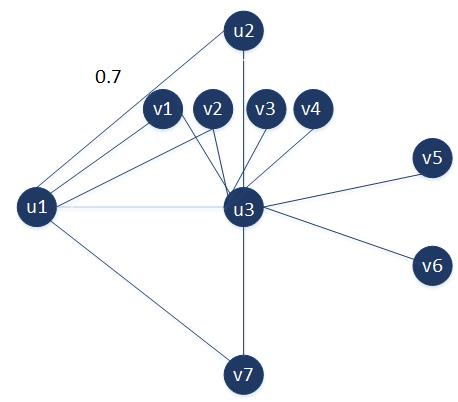
\includegraphics[width=80mm]{common_neighbors.jpg}
	\caption{Ryšių grafo fragmentas} \label{common_neighbors}
\end{figure}

\ref{common_neighbors} pav. pavaizduotas socialinio tinklo fragmentas, kuriame žinomas tik $u_2$ pasitikėjimas $u_1$, kuris šiame pavyzdyje yra lygus $0.7$. Tarkime, kad norime įvertinti $t_{u_3}(u_1)$. Iš grafo matosi, kad $r(u_1)=4$, $r(u_3) = 7$ ir $br(u_1,u_3)=3$ ($u_1$ turi ryšį su 4 naudotojais, $u_1$ - su $7$, o šių naudotojų bendrų ryšių skaičius - $3$). Žinodami, kad $t_{u_2}(u_1) = 0.7$, galime teigti, kad $t_{u_3}(u_1)$ tikrai nebus didesnis nei $t_{u_2}(u_1)$, nes trūkstamas propagavimo kelio pasitikėjimo įvertis $t_{u_3}({u_2})$ nebus didesnis už $1$. Jį galima įvertinti jau minėta taisykle \ref{rule:sim} .
Kitas būdas - spręsti skaitinės prognozės uždavinį. Naudojant mokymo duomenis būtų galima įvertinti sąryšį tarp bendrų ryšių skaičiaus ir pasitikėjimo įverčio. Mokymo duomenys – matrica pavidalo 
\begin{displaymath}
[ \boldsymbol{R_1}, \boldsymbol{R_2}, \boldsymbol{BR}, \boldsymbol{Y}]
\end{displaymath}
Čia $\boldsymbol{R_1}$ ir $\boldsymbol{R_2}$ - naudotojų porų, kurioms žinomas tarpusavio pasitikėjimas, ryšių skaičiaus vektorius, $\boldsymbol{BR}$ - jų bendrų ryšių skaičiaus vektorius, o $\boldsymbol{Y}$ - priklausomas žinomo pasitikėjimo įverčio tarp jų vektorius. Testuoti gautus rezultatus galima prognozuojant reitingus ir taikant prognozės tikslumo matus, aprašytus kitame skyriuje.

\subsection{Sričių panašumo metodas}

Šalto starto sąvoka nėra vienareikšmiškai apibrėžiama - negalime iš anksto žinoti, kiek ir kokių reikia duomenų, kad situacija tenkintų apibrėžimą ir taikomas metodas veiktų kaip tikimąsi. Aplinkoje, apie kurią dabar rašoma, naudotojas gali būti šalto starto padėtyje, kai kalbame apie vieną sritį, tačiau kitoje srityje padėtis gali būti priešinga. Kitaip tariant, jeigu norime sužinoti, koks yra $t_a^2(b)$, ir žinome, kad naudotojo $u_1$ pasitikėjimo naudotoju $u_2$ srityje $T_1$ lygis yra $0.8$, o $s^d(T_1, T_2) = 0.9$, nieko nežinodami apie naudotojų santykį $T_2$ klausimu, galime įvertinti jų tarpusavio pasitikėjimą tiesiog padauginę žinomos srities pasitikėjimo įvertį iš sričių tarpusavio panašumo įverčio.
\newline
\indent
Ši idėja yra pritaikoma ne tik šalto starto atveju, kai kalbama apie naudotoją, bet ir naujos srities šalto starto atveju. Socialinius tinklus pagal pasitikėjimo sričių daugialypiškumą galima išskirti į du tipus:
\begin{itemize}
	\item daugiaprofilinius - juose galimos įvairios pasitikėjimo sritys - tokios, kurias galima surikiuoti pagal panašumą ir tarp pirmos bei paskutinės nėra jokio panašumo.
	\item specializuotos - juose pasitikėjimo sritys yra gana artimos. Tokio tinklo pavyzdys galėtų būti kino mėgėjų socialinis tinklas, o sritys - įvairūs žanrai. 
\end{itemize}
Siūlomas metodas tinka abiems tipams, tačiau pirmojo tipo atveju, dėl platesnio išsibarstymo pasitikėjimo skalėje, gali būti ypač naudingas.
\begin{figure}[ht!]
	\centering
	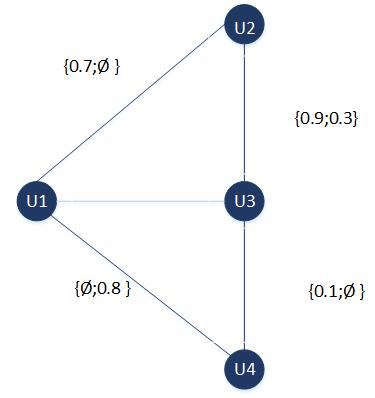
\includegraphics[width=60mm]{multiarea.jpg}
	\caption{Ryšių grafo fragmentas} \label{multiarea}
\end{figure}
Tarkime, kad turime situaciją pavaizduotą grafe \ref{multiarea}, kuriame pateikti naudotojų tarpusavio pasitikėjimai ${t_1, t_2}$, ir norime žinoti, kiek $u_1$ pasitiki $u_3$ dėl $T_2$. Tiesioginio būdo nėra, nes abiejuoe galimuose keliuose - $u_1 - u_2 - u_3$ ir $u_1 - u_4 - u_3$ yra trūkstamų duomenų - pirmu atveju nežinome $t_{u_1}^2(u_2)$, antru - $t_{u_4}^2(u_3)$, tačiau matome, kad egzistuoja kelias $u_1 - u_2 - u_3$, pagal kurį galime įvertinti $t_{u_1}^1(u_3)$
\begin{displaymath}
t_{u_1}^1(u_3)=t_{u_1}^1(u_2) \times t_{u_2}^1(u_3) = 0.7 \times 0.9 = 0.63
\end{displaymath}
Žinodami, kad sričių panašumas $s^d(T_1, T_2) = 0.9$, gauname
\begin{displaymath}
t_{u_1}^1(u_3)=t_{u_1}^1(u_3) \times s^d(T_1, T_2) = 0.63 \times 0.9 = 0.6048
\end{displaymath}
Panašumą tarp sričių galime priskirti \it{ad hoc} \normalfont arba įvertinti vienu iš šių būdų:
\begin{itemize}
	\item Tarkime, kad turime naudotojų porų sąrašą ir jų tarpusavio pasitikėjimą (arba panašumą) pagal sritis. Tada:
	\begin{displaymath}\label{eq:areasim}
	s^d(T_1, T_2) = \frac{\sum \limits_{i=1}^n \frac{\min(t_{u_i}^1, t_{u_i}^2)}{\max(t_{u_i}^1, t_{u_i}^2)}}{n}
	%s^d(T_1, T_2) = average \bigg(\frac{min(\boldsymbol{t}_1, \boldsymbol{t}_2)}{max(\boldsymbol{t}_1, \boldsymbol{t}_2)}\bigg) 
	\end{displaymath}
	\indent
	Kitas būdas:
	\begin{displaymath}\label{eq:areasim}
	s^d(T_1, T_2) = 1-\frac{\sum \limits_{i=1}^n \big[\max(t_{u_i}^1, t_{u_i}^2)- \min(t_{u_i}^1, t_{u_i}^2)\big]}{n}
	%s^d(T_1, T_2) = average \bigg(\frac{min(\boldsymbol{t}_1, \boldsymbol{t}_2)}{max(\boldsymbol{t}_1, \boldsymbol{t}_2)}\bigg) 
	\end{displaymath}
	\item Kitas būdas - taikyti vieną iš panašumo radimo metodų (Pyrsono, Spearmano koreliacija, kosinuso panašumas) turimiems pasitikėjimo (arba panašumo) duomenims. Verta pastebėti, kad šis metodas palyginus su anksčiau pasiūlytais yra griežtesnis ir grąžina mažesnį panašumą.
\end{itemize} 
\subsection{Pasitikėjimo apskaičiavimas pasitikėjimo sritims taikant tiesinę regresiją}\label{ssec:linreg}
Praeitame skyrelyje pasiūlytas metodas turi stiprų loginį pagrindimą - idėja, kad žinant pasitikėjimo tam tikroje srityje įvertį ir panašumą tarp sričių, galime konservatyviai prognozuoti pasitikėjimą kitoje srityje, atrodo intuityviai suprantama. Į šią problemą galima pažvelgti ir iš statistinės perspektyvos. Norime įvertinti naudotojo $u_j$ pasitikėjimą naudotoju $u_k$ srityje $T_2$. Turime duomenis $\{(t_{u_j}^1(u_{p_1}), t_{u_j}^2(u_{p_1})),... , (t_{u_j}^1(u_{p_k}), t_{u_j}^2(u_{p_k}))\}, k \in \bar{1,N} $ ir $t_{u_i}^1(u_j)$. Kadangi nežinomas įvertis antroje pasitikėjimo srityje $T_2$, ją įvardiname kaip regresorių, o $T_1$ - predikatą.

\begin{figure}[ht!]
	\centering
	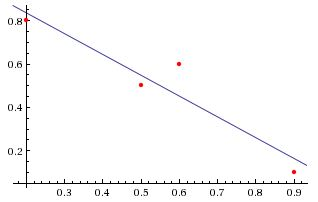
\includegraphics[width=80mm]{linreg.jpg}
	\caption{Tiesinė regresija} \label{linreg}
\end{figure}
Norint įvertinti $t_{u}^i(v)$, kur $i$ - pasitikėjimo srities indeksas, reikia žinoti pasitikėjimo įverčius visoms dimensijoms (išskyrus tą, kurią norime įvertinti) tam tikram naudotojų kiekiui. Jau anksčiau buvo kalbėta apie duomenų retumo problemą - natūralu, kad ir šiuo atveju pilno duomenų rinkinio niekada neturėsime.

\begin{center}
	\captionof{table}{Naudotojo $u$ pasitikėjimas aštuoniais naudotojais keturiose pasitikėjimo srityse}
	\begin{tabular}{ | l | l | l | l | l |}
		\hline
		 & $T_1$ & $T_2$ & $T_3$ & $T_4$\\ \hline
		$\boldsymbol{t}_u(v_1)$ & 0.7 & 0.4 &  & \\ \hline
		$\boldsymbol{t}_u(v_2)$ &  &  & 0.7 & \\ \hline
		$\boldsymbol{t}_u(v_3)$ &  & 0.6 &  & \\ \hline
		$\boldsymbol{t}_u(v_4)$ & 0.6 & ? & 0.4 & 0.5\\ \hline
		$\boldsymbol{t}_u(v_5)$ & 0.8 & 0.3 &  & \\ \hline
		$\boldsymbol{t}_u(v_6)$ &  &  & 0.9 & \\ \hline
		$\boldsymbol{t}_u(v_7)$ &  &  &  & 0.8\\ \hline
		$\boldsymbol{t}_u(v_8)$ & 0.9 & 0.4 &  & 0.9 \\\hline
		\hline
	\end{tabular}
\end{center}
Vienas būdų, kaip įvertintį norimą pasitikėjimą - parinkti tam tikras dimensijas, kurioms tada taikoma tiesinė regresija. 
\begin{itemize}
	\item nustatome mus dominantį naudotoją ($v_4$)
	\item nustatome, kurioms sritims mus dominantis naudotojas turi pasitikėjimo įverčius.($T_1, T_3, T_4$)
	\item atrenkame naudotojų, kurie turi pasitikėjimo įverčius mus dominančiai sričiai, aibę ($v_1$, $v_2$, $v_3$, $v_5$, $v_8$)
	\item einame per pasitikėjimo sritis ir žiūrime, kiek naudotojų iš atrinktos aibės turi įverčius konkrečiai sričiai ($T_1$ - $4$, $T_3$ - $3$, $T_4$ - $3$)
	\item atrenkame tuos naudotojus, kurie turi įverčius sričiai, kuri turėjo daugiausiai įverčių praeitame žingsnyje ($v_1$, $v_4$, $v_5$, $v_8$)
	\item taikome tiesinę regresiją atrinktų naudotojų duomenimis atrinktoms sritims
\end{itemize}
Pavyzdyje pateiktiems duomenims, taikytume tiesinę regresiją dimensijoms $T_1$, $T_2$, o duomenų aibę sudarytų naudotojų $v_1$, $v_4$, $v_5$, $v_8$ duomenys.
\newline
\indent
Šį metodą galima palyginti su anksčiau pasiūlytu sričių panašumo metodu nagrinėjant tam tikrą ribinį atvejį. Turime naudotojo $u$ ir kitų keturių naudotojų tarpusavio pasitikėjimą dviejose srityse. Duomenys tokie: 
\begin{displaymath}
t_{u}^1(v_1)=0; t_{u}^2(v_1)=0
\end{displaymath}
\begin{displaymath}
t_{u}^1(v_2)=0; t_{u}^2(v_2)=1
\end{displaymath}
\begin{displaymath}
t_{u}^1(v_3)=1; t_{u}^2(v_3)=0
\end{displaymath}
\begin{displaymath}
t_{u}^1(v_4)=1; t_{u}^2(v_4)=1
\end{displaymath}
Tokiu atveju, sričių panašumo metodas identifikuoja, kad panašumas tarp sričių lygus 0 ir net jei žinome, kiek $u$ pasitiki naudotoju bet kurioje srityje, nieko negalime pasakyti apie pasitikėjimą kitoje. Tiesine regresija paremtas metodas esant bet kokiam pasitikėjimui vienoje srityje, teigtų, kad pasitikėjimas kitoje yra $0.5$. Taigi, abu metodai, iš esmės sako, kad jie nieko nežino - pirmas atsisako vertinti visai, kitas vertina $50 - 50$, ir abu jie yra savaip teisūs. 
\newline
\indent
 Šį metodą prasminga taikyti ne visada, o tik esant sąlygai, kad egzistuoja tam tikras ryšys tarp pasitikėjimo sričių. Tyrimu galima nustatyti, koks turi būti sričių panašumas, kad tiesinės regresijos taikymas būtų prasmingas. Regresijos tiesės nuolydis priklauso ir nuo paties naudotojo santykiu su pasitikėjimo sritimis. Galima iškelti tokią hipotezę: tarkime, yra 2 panašios sritys, tačiau naudotojas $u$ srityje $T_1$ jaučiasi nusimanąs labiau nei $T_2$. Tada, žmonės, kuriais jis pasitiki srityje $T_1$ labiau, turės dar didesnius pasitikėjimo įverčius srityje $T_2$, o tai reikš, kad regresijos tiesės koeficientas bus didesnis už 1. Šios hipotezės patvirtinimas arba paneigimas - psichologijos tyrimų objektas.

\subsubsection{Pasitikėjimo kryptis}
Iki šiol nebuvo akcentuota pasitikėjimo krypties sąvoka - visuose pavyzdžiuose darėme prielaidą, kad pasitikėjimas turi kryptį ir nėra abipusis. Tačiau galima išskirti du RS tipus, pagal tai, kur kryptingumas yra svarbus ir kur galima daryti prielaidą, kad $t_u(v)= t_v(u)$.
\begin{itemize}
	\item kryptingumas yra svarbus, tinkluose, kur pasitikėjimas reiškia pasitikėjimą kaip specialistu (pavyzdžiui, $u$ pasitiki $v$ kaip debesų kompiuterijos specialistu, tačiau pats yra naujokas šioje srityje, todėl atvirkščias teiginys negalioja)
	\item kryptingumas nėra toks svarbus, tinkluose, kur pasitikėjimas reiškia, kiek panašūs skoniai (pavyzdžiui, $u$ patiko panašūs filmai kaip ir $v$, todėl būtų pagrįsta manyti, kad ir $v$ patiks panašūs filmai kaip ir $u$)
\end{itemize}
Anksčiau buvo minėta, kad pasitikėjimas turi kryptį - naudotas $u$ pasitiki naudotoju $v$ nebūtinai tiek pat, kiek $v$ pasitiki $u$. Tačiau šalto starto atveju, galima daryti prielaidą, kad $\boldsymbol{t}_u(v) = \boldsymbol{t}_v(u)$. Tada ir metodas, naudojantis tiesinę regresiją gali būti klasifikuojamas kaip sprendžiantis šalto starto problemą.
\newline
\indent
Metodas, naudojantis tiesinę regresiją pagal savo esmę labiau tinka vertinti naudotojo, turinčio daug duomenų pasitikėjimą naudotoju, turinčiu mažai duomenų. Tačiau, remiantis idėja apie pasitikėjimo krypties nebuvimą, galime vertinti atvirkščiai, ir tokiu būdu spręsti šalto starto problemą.

%\subsection{Vertinimas}
%\section{Pasiekti rezultatai}
\section{Tyrimas}
\subsection{Bendrų kaimynų metodas}
Dalis tyrimo (nereikalaujanti duomenų apie naudotojų tarpusavio pasitikėjimą kategorijų lygmenyje) buvo atlikta naudojant viešai prieinamą Epinions.com duomenų rinkinį. Šio duomenų rinkinio struktūra tokia:
\begin{itemize}
	\item naudotojai
	\begin{itemize}
		\item naudotojo id
	\end{itemize}
	\item reitingai
	\begin{itemize}
		\item naudotojo id
		\item elemento id
		\item reitingas
	\end{itemize}
	\item pasitikėjimai
	\begin{itemize}
		\item naudotojo id
		\item naudotojo id
	\end{itemize}
\end{itemize}
\indent
Panašumas buvo skaičiuojamas taikant šiuos panašumo matus:
\begin{itemize}
	\item Pyrsono koreliacija
	\item Spearmano koreliacija
	\item Kosinuso panašumas
\end{itemize}
\indent
Šio tyrimo tikslas – ištirti pasiūlytų metodų efektyvumą ir tikslumą sprendžiant šalto starto problemą rekomendacinėse sistemose. Tikslumas vertinamas naudojant "išimk vieną" metodą, kurio esmė tokia - iš duomenų išimamas vienas reitingas ir tada bandoma jį prognozuoti remiantis likusiais sistemos duomenimis. Tada tikslumas matuojamas taikant vieną iš šių matavimo būdų:
\begin{itemize}
	\item Vidutinė absoliuti klaida (angl. mean absolute error)
	\begin{equation}
	MAE = \sqrt{\frac{1}{|T|}\sum\limits_{(u,i)\in T} |\hat{r}_{ui} - r_{ui}|}
	\end{equation}
	\item Vidutinė absoliuti naudotojo klaida (angl. mean absolute user error) – vidutinė absoliuti klaida skaičiuojama kiekvienam naudotojui atskirai, o tada randamas tų klaidų vidurkis.
	\item Kvadratinė vidutinė klaida (angl. root mean squared error)
	\begin{equation}
	RMSE = \sqrt{\frac{1}{|T|}\sum\limits_{(u,i)\in T} (\hat{r}_{ui} - r_{ui})^2}
	\end{equation}
\end{itemize}

%predictions
%table MAE, MAUE, RMSE/ Similarity measures

\indent
Siūlomų metodų rezultatai vertinami lyginant su rezultatais, gautais taikant tradicinį bendradarbiavimo filtravimo metodą. Šis metodas gali būti taikomas naudojant skirtingus panašumo matus. Tyrimas buvo atliktas prognozuojant $608603$ reitingus nuo $35685$ naudotojų. Atlikus anksčiau apibrėžtų kriterijų vertinimą, gauti tokie rezultatai.
\begin{center}
	\captionof{table}{Bazinio metodo taikymo rezultatai}
	\begin{tabular}{ | l | l | l | l |}
		\hline
		& $MAE$ & $MAUE$ & $RMSE$ \\ \hline
		Pyrsono koreliacija   & 0.859 & 0.889 & 1.031 \\ \hline
		Spearmano koreliacija & 0.860 & 0.892 & 1.04  \\ \hline
		Kosinuso panašumas    & 0.902 & 0.923 & 1.063  \\ \hline
		\hline
	\end{tabular}
\end{center}
Taikant Pyrsono ir Spearmano koreliaciją gauti rezultatai labai panašūs, kosinuso panašumo - prastesni. Dėl šios priežasties toliau bus remiamasi tik Pyrsono koreliacija.
\subsection{Sričių panašumo metodas}
\indent
Šiuo metu nėra viešai prieinamo duomenų rinkinio tobulai tinkančio atliekamam tyrimui.  Kaip minėta anksčiau, turimi pasitikėjimo tarp naudotojų įverčiai lygūs $1$. Kadangi šiame tyrime norima parodyti metodo, naudojančio tolydžius duomenis efektyvumą, pasitikėjimo įverčiai tarp naudotojų proporcingai priskiriami panašumo įverčiams, gautiems taikant Pyrsono koreliaciją. Naudotojų poroms, kurioms koreliacijos dėl bendrai įvertintų elementų nebuvimo nustatyti nepavyko, pasitikėjimas prilygintas $0.4$ - panašumų vidurkiui. Verta paminėti, kad prielaida apie pasitikėjimo proporcingumą panašumui yra gana grubi. Iš tiesų, įvertinus pasitikinčių naudotojų porų panašumą, paaiškėjo, kad $16.8\%$ panašumas buvo neigiamas o vidurkis yra tik  $0.43$. Nors šis dydis naudojamas tik kaip svoris ir jo absoliuti reikšmė įtakos neturi, tai byloja apie tam tikrą naudotojų neracionalumą identifikuojant jiems patikimus naudotojus. 
\indent
Įyrimas buvo atliekamas dviem lygiais - globaliu, kuriame kalbama apie naudotojų pasitikėjimą sistemoje visose srityse ir kategorijų lygiu. Turimo epinions.com duomenų rinkinio karegorijų struktūra susideda iš xxx kategorijų, išsidėsčiusio 4-iais lygiais. (pav.) Tokia struktūra šiam tyrimui yra per smulki - būtų sunku apskaičiuoti panašumą tarp naudotojų skirtingose tokio smulkumo kategorijose. Dėl šios priežasties kategorijos buvo "suplokštintos", taigi pavyzdžiui elementas priklausęs kategorjai "Video žaidimai" buvo priskirtas kategororijai "Žaidimai" ir panašiai. Kai visi elementai buvo  priskirti vieno lygio kategorijoms, buvo apskaičiuoti panašumai tarp naudotojų atskirtose kategorijose. Tam, kad tarp naudotojų būtų įnamona rasti panašumą, reikia, kad jie pasirinktoje kategorijoje bendrai būtų įvertinę keturis ar daugiau tų pačių elementų. Atlikus tyrimą, paaiškėjo, kad tokią salyga gana sunku patenkinti dėl didelio elementų skaičiaus ir per mažo naudotojų aktyvumo vertinant elementus.
\newline
\indent
Kaip dalis duomenų parengimo etapo gali būti vertinamas ir pagrindinių operatorių - propagavimo ir agregavimo - taikymas turimiems duomenims. Dauguma anksčiau pristatytų tyrimų apie šalto starto problemą rekomendacinėse sistemose taikant socialinių tinklų duomenis [tokie ir tokie] kalbėjo būtent apie tai, kaip padidinti reikalingų pasitikėjimo duomenų kiekį taikant propagavimo ir agregavimo operatorius. Šiuo tyrimu siekiama eiti toliau - panaudoti ankstesnius darbus kaip pagrindą. Nors Golbeck disertacijoje išsamiai aprašytas TidalTrust algoritmas atrodo teoriškai pagrįstas, igyvendinti jį praktikoje pasirodė gana sudėtinga. Šiame tyrime propaguoti pasitikėjimai buvo apskaičiuoti taikant trumpiausio kelio algoritmą, kurio esmė rasti trumpiausią pasitikėjimo kelią tarp dviejų naudotojų ir sudauginus pasitikėjimo iverčius, rasti naują įvertį. Taikant šį metodą pasitikėjimą buvo galima buvo įvertinti didžiajai daugumai naudotojų porų (dėl grafo jungumo), tačiau mus domina tik pasitikėjimai, kurie savyje turi vertiną informaciją, tai yra, nuo tam tikro slenksčio. [Tyrimas]
\subsection{Bendrų kaimynų metodas}
\subsubsection{Globalus bendrų kaimynų metodas}
\indent
Metodų efektyvumą sprendžiant šalto starto problemą vienareikšmiškai įvertinti ir palyginti neįmanoma dėl to, kad kiekvienas metodas taikomas skirtingose situacijose. Bendrų kaimynų metodą prasmingiausia taikyti, kai žinomi tik naudotojo ryšiai su kitais naudotojais. Dėl to, kad ši informacija nėra išgaunama iš tikrų reitingų, šio metodo tikslumas gali būti mažesnis negu tradicinio bendradarbiavimo filtravimo.
\newline
\indent
Taikant bendrų kaimynų metodą, yra svarbūs naudotojų ryšių ir bendrų ryšių skaičiai. Buvo sudaryta duomenų matrica pavidalo $[ \boldsymbol{R_1}, \boldsymbol{R_2},  \boldsymbol{Y}]$, kur $\boldsymbol{R_1}$ ir $\boldsymbol{R_2}$ - naudotojų $u_1$ ir $u_2$ bendrų tarpusavio ryšių skaičiaus santykis su naudotojų $u_1$ ir, atitinkamai, $u_2$ ryšių skaičiumi, o $\boldsymbol{Y}$ - prognozuojamas pasitikėjimas. Mokymo imtį sudaro naudotojų $201542$ poros, kurioms duomenų paruošimo etape pavyko įvertinti panašumą ir kurios turi vieną arba daugiau bendrą ryšį. Šiems duomenims pritaikius tiesinę regresiją, gauta tokia formulė:
\begin{equation}\label{eq:CN_all}
y = 0.046 \times r_1 + 0.021 \times r_2 + 0.406
\end{equation}
Akivaizdu, kad koeficientai yra gana maži. Tai gali rodyti, kad pirminė prielaida apie sąryšį tarp pasitikėjimo ir bendrų ryšių skaičiaus - naudotojo ryšių skaičiaus santykio šiems duomenims nepasitvirtino. Tačiau parinkę kitokią naudotojų imtį - tokią, apie kurią turime daugiau informacijos, šiuo atveju su didesniu bendrų ryšių skaičiumi, gauname kiek kitokį vaizdą. Parinkę naudotojų poras, kurios turi daugiau negu 150 bendrų ryšių (tokių yra 634), gauname tokią formulę:
\begin{equation}\label{eq:CN_150}
y = 0.356 \times r_1 + 0.366 \times r_2 + 0.0644
\end{equation}
\newline
Iš tiesų tokia imtis aiškiau leidžia įžvelgti priklausomybę tarp bendrų ryšių. Rezultatai rodo, kad tiek $r_1$, tiek $r_2$ yra vienodai svarbūs.
\indent
\begin{figure}[ht!]
	\centering
	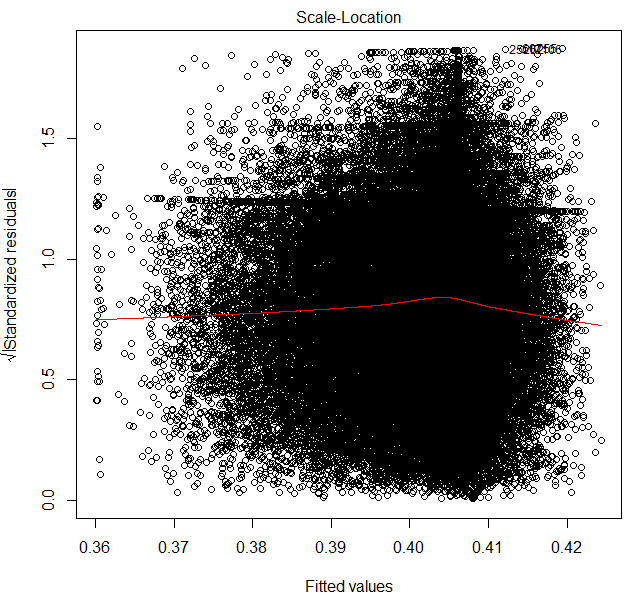
\includegraphics[width=80mm]{CN_residuals.png}
	\caption{Pasitikėjimo prognozių ir standartizuotų liekanų taškinė diagrama} \label{CN_residuals}
\end{figure}
\begin{figure}[ht!]
	\centering
	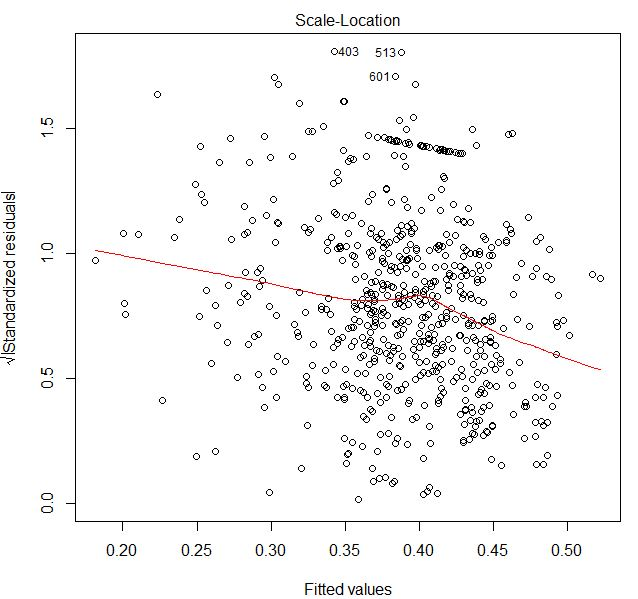
\includegraphics[width=80mm]{CN_residuals_150.jpg}
	\caption{Pasitikėjimo prognozių ir standartizuotų liekanų taškinė diagrama daugiau nei 150 bendrų ryšių turinčioms naudotojų poroms} \label{CN_residuals_150}
\end{figure}
Pav. \ref{CN_residuals} pavaizduotame grafike matosi prognozės ir šaknies iš standartizuotų liekanų taškinė diagrama. Dėl mažų regresijos koeficientų pasitikėjimo prognozės yra išsidėsčiusios mažame intervale, o liekanos - gana didelės. Prognozės tikslumas mažiausias apie vidurkį - tai yra toms naudotojų poroms, kurios turėjo mažą bendrų - savo ryšių skaičiaus santykį, tai yra tiems, apie kuriuos buvo žinoma mažiausiai. Pav. \ref{CN_residuals_150} vaizdas kiek kitoks. Naudotojų poroms, kurioms prognozuotas mažesnis pasitikėjimas pastebimas mažesnis prognozės tikslumas. Kuo mažesnis pasitikėjimas prognozuojamas, tuo yra mažesnis bendrų draugų skaičiaus ir draugų skaičiaus santykis. Kaip ir tikėtasi, prognozė geriausiai veikia naudotojams, kurie turi didžiausias $r_1$ ir $r_2$ reikšmes.
\newline
\indent
Remiantis gautomis formulėmis buvo įvertintas pasitikėjimas, o tuomet pritaikius bendradarbavimo filtravimą, naudojant gautus įverčius, prognozuoti naudotojų įvertinimai. Rezultatai lyginami su rezultatais, gautais taikant bendradarbiavimo filtravimą pradiniams pasitikėjimo duomenims. Imtis - atsitiktinai parinkta 2000 naudotojų aibė. 
\begin{center}
	\captionof{table}{Bendrų kaimynų metodo taikymo rezultatai}
	\begin{tabular}{ | l | l | l | l | }
		\hline
		Metodas taikomas pasitikėjimui rasti & $MAE$ & $MAUE$ & $RMSE$\\ \hline
		 Pasitikėjimas (Pyrsono koreliacija)        & 0.902 & 0.913 & 1.167  \\ \hline
		 Pasitikėjimo prognozė taikant \ref{eq:CN_all}	  					& 0.913 & 0.905 & 1.182  \\ \hline
		 Pasitikėjimo prognozė taikant \ref{eq:CN_150} 					& 0.8900 & 0.91329 & 1.114  \\ \hline
		\hline
	\end{tabular}
\end{center}

Skirtumas tarp $MAE$ ir $RMSE$ rezultatų gautų taikant bendrų kaimynų metodą nuo bazinių rezultatų skiriasi nežymiai. Geriausi rezultatai pagal MAE ir RMSE gauti naudojant prognozę, sudarytą remiantis daugiausiai ryšių turinčių naudotojų imtimi. Šiek tiek didesnis $MAUE$ skirtumas. Taip yra dėl to, kad naudotojai turi nevienodą skaičių reitingų ir $MAUE$ atsižvelgia į tai. Vadinasi, bendrų kaimynų metodas sudarė prognozes mažiau reitingų turėjusiems naudotojams su mažesniu tikslumu negu bazinis bendradarbiavimo filtravimo metodas.


%common neighbours
%table MAE, MAUE, RMSE/ Similarity measures

\subsection{Sričių panašumo metodas}
\subsubsection{Duomenų generavimas}
\indent
Anksčiau buvo minėta, kad šiuo metu nėra tokio duomenų rinkinio, tinkančio atliekamam tyrimui. Dėl šios priežasties dalis tyrimo skirta modelio sudarymui ir duomenų generavimui. Siekiama sukurti duomenų struktūrą, turinčią tokius elementus:
\begin{itemize}
	\item Kategorijos
	\item Naudotojai
	\item Elementai (reitinguojami produktai) priklausantys kategorijoms
	\item Naudotojo tarpusavio pasitikėjimai kategorijose (tolydi reikšmė tarp 0 ir 1)
	\item Naudotojų reitingai priskirti elementams
\end{itemize}
Toliau bus aprašyti kiekvieno iš elementų generavimo algoritmai.
\subsubsubsection{Kategorijos}
Kategojų modeliavimas - pirmas algoritmo žingsnis. Juo siekiama apibrėžti ne tik kategorijas, kurioms gali priklausyti elementai bet ir kiekvieno elemento bruožus bei kiekvieno naudotojo pirmenybes. Šiame tyrime generuojami duomenys gali būti traktuojami kaip filmų rekomendacinės sistemos duomenys. Apibrėžiame kategorijas:
\begin{itemize}
	\item $X_1$ - drama
	\item $X_2$ - komedija
	\item $X_3$ - siaubo
	\item $X_4$ - trileris
	\item $X_5$ - fantastika
\end{itemize}
Toliau apibrėžiame, kiek kiekviena iš šių kategorijų yra susijusi su kitomis. Heuristiškai sudarome matricą:
\begin{center}
	\begin{tabular}{||c c c c c c||} 
		\hline
		Kategorijos & $X_1$ & $X_2$ & $X_3$ & $X_4$ & $X_5$ \\ [0.5ex] 
		\hline\hline
		$x_1$ & 0.55 & 0.2 & 0.2 & 0.2 & 0.3 \\ 
		\hline
		$x_2$ & 0.2 & 0.6 & 0.05 & 0.05 & 0.1 \\
		\hline
		$x_3$ & 0.05 & 0.05 & 0.35 & 0.1 & 0.05 \\
		\hline
		$x_4$ & 0.1 & 0.05 & 0.2 & 0.65 & 0.05 \\
		\hline
		$x_5$ & 0.1 & 0.1 & 0.2 & 0 & 0.5 \\ [1ex] 
		\hline
	\end{tabular}
\end{center}
Čia $X_1, .., X_5$ žymime kategorijas, o $x_1, .., x_5$ kategorijas atitinkančius požymius. Taigi iš šios matricos galime teigti, kad pavyzdžiui:
\begin{itemize}
	\item $X_4$ (trileris) yra gryniausias žanras, tai yra, turintis daugiausiai savo kategoriją atitinkančio požymio (kadangi turi didžiausią matricos įstrižainėje esančią reikšmę)
	\item $X_3$ (siaubo) - mažiausiai gryna kategorija (nes bruožų pasiskirstymas yra tolygiausias)
	\item $X_4$ kategorija neturi $x_5$ bruožo (trileris neturi fantastikos)
\end{itemize} 
Akivaizdu, kad šie teiginiai yra subjektyvūs. Didesnio objektyvumo galima pasiekti atliekant apklausas.

\subsubsubsection{Naudotojai}
\indent
Naudotojas apibrėžiamas kaip vektorius $(y_1, y_2, y_3, y_4, y_5, q)$, kur $\sum\limits_{i=1}^{5} y_i = 1$ ir $q\in[0,1]$. $y_1, y_2, y_3, y_4, y_5$ reiškia naudotojo pirmenybes - kiek svarbus jam yra tam tikras bruožas elemente.
$q$ - kokybės parametras rodo, kiek naudotojas yra jautrus elemento kokybei. Metafora iš realaus gyvenimo - net jei žmogui apskritai nepatinka siaubo filmai, egzistuoja bent vienas kurį jis vertintų labai gerai (dėl to, kad tas filmas yra aukštos kokybės ir patinka daugumai). 
\newline
\indent 
Praktiškai algoritmas realizuojamas taip:
\begin{itemize}
	\item sugeneruojame 5 atsitiktinius skaičius tarp 0 ir 1 (naudojant tolygų skirstinį)
	\item randame jų sumą
	\item kiekvienam bruožui priskiriame reikšmę lygią pirmame žingsnyje sugeneruotai reikšmei padalintai iš visų reikšmių sumos
	\item kokybės parametrui priskiriame atsitiktinę reikšmę tarp 0 ir 1
\end{itemize}
Taip užtikriname, kad naudotojai yra tikrai atsitiktiniai ir įvairūs pirmenybių prasme.
\subsubsubsection{Elementai}
\indent
Elementas apibrėžiamas vektoriumi $(c, z_1, z_2, z_3, z_4, z_5, q)$. Čia $z_1, z_2, z_3, z_4, z_5$ rodo, kiek elementas pasižymi kiekvienu bruožu, o $q$ - kokybės parametras. $c$ - rodo, kuriai karegorijai priklauso elementas. Negalime taikyti tokio paties metodo, kaip naudotojo atveju, nes elementas priklauso vienai kategorijai, o tai reiškia, kad bruožų reikšmės negali būti visiškai atsitiktinės. Bruožų reikšmes generuojame pasinaudodami normaliuoju skirstiniu su vidurkiu lygiu reikšmei gautai iš kategorijų matricos, aprašytos skyrelyje apie kategorijas ir parinkta dispersija (tokia, kad duomenys būtų panašūs į realius - parinkus per didelę dispersiją rezultatai gaunasi labai triukšmingi). Vidurkis parenkamas taip: pažiūrėję į $c$ reikšmę atfiltruojame kategoriją (stulpelį). Tada turime vidurkių, naudojamų generuojant $z_1, z_2, z_3, z_4, z_5$, vektorių. Kokybės parametras, kaip ir naudotojo atveju, parenkamas atsitiktinai pagal normalųjį skirstinį su vidurkiu $0.6$ ir dispersija lygia $0.4$. Jei sugeneruota reikšmė didesnė už 1 arba mažesnė už 0, ji priskiriama 1 arba 0 atitinkamai.
\subsubsubsection{Reitingai}
\indent
Naudotojo reitingai elementams generuojami naudojant naudotojo pirmenybes ir reiklumo kokybei parametrą bei atitinkamus produkto parametrus. Siekiama, kad jų pasiskirstymas būtų kuo artimesnis tikrovei, tai jie nebūtų pasiskirstę galimų reikšmių kraštuose ir nebūtų pernelyg vienodi. Sugeneruotų duomenų charakteristikos bus pateiktos kitame skyrelyje. 
\newline
\indent
Kiekvienam naudotojui parenkamas atsitiktinis įvertintų elementų skaičius naudojant atsitiktinį dydį pasiskirsčiusį pagal normalųjį skirstinį su vidurkiu 30 ir dispersija 27. Parinkta didelė dispersija užtikrina, kad duomenys bus artimesni tikriems - Epinions.com duomenų rinkinyje vieno naudotojo įvertintų elementų skaičius svyruoja nuo 0 iki 655. Kiekvienam atsitiktinai parinktam elementui generuojamas reitingas tokiu būdu:
\begin{equation}
	r_u(p) = 5 \times ((1-q_u) \sqrt{pos(corr(X_u,Y_p))} + q_u q_p)
\end{equation}
čia
\begin{itemize}
	\item $r_u(p)$ - naudotojo $u$ reitingas elementui $p$
	\item $q_u$ - naudotojo $u$ kokybės reiklumo parametras
	\item $q_p$ - elemento $p$ kokybės parametras
	\item $X_u$ - naudotojo $u$ primenybių rinkinys 
	\item $Y_p$ - elemento $p$ bruožų rinkinys
	\item $pos(x)$ - $f[-1,1] -> [0,1]$
\end{itemize}
\indent
Idealiais atvejais, kai naudotojo reiklumas kokybei ir elemento kokybė lygi 1 arba naudotojo reiklumas kokybei lygus 0, tačiau elemento charakteristikos tobulai atitinka anudotojo pirmenybes, reitingas lygus 5. Tyrimo eigoje pastebėta, kad koreliacijos funkcijos įtaka pernelyg maža, todėl ji padidinama iškilia funkcija (šiuo atveju šaknis suteikia pageidaujamą efektą).
\subsubsubsection{Pasitikėjimai}
\indent
Pasitikėjimo reikšmės - svarbiausios prognozuojant reitingus, parodančios kokį svorį suteikti patikėtinio nuomonei apie elementą. Šiame tyrime naudotojai vieni kitais pasitiki kategorijos lygmenyje. Buvo išbandyti du pasitikėjimo reikšmių generavimo būdai.
\newline
\indent
Taikant pirmąjį būdą pasitikėjimas tarp dviejų naudotojų tam tikroje kategorijoje generuojamas lyginant naudotojų tarpusavio pirmenybes tos kategorijos atžvilgiu. Taigi pasitikėjimas kategorijoje $X_1$ tarp naudotojų $u(0.1, 0.2, 0.2, 0.5, 0, q_u)$ ir $v(0.2, 0.2, 0.2, 0.2, 0.2, q_v$ randamas taip:
\begin{equation}
	t_u(v) = \frac{min(x_1^u, x_1^v)}{max(x_1^u, x_1^v)} = \frac{0.1}{0.2} = 0.5
\end{equation}
Tokiu būdu rasti pasitikėjimai tenkina šias savybes:
\begin{itemize}
	\item yra intervale tarp 0 ir 1
	\item nepriklauso nuo kategorijų skaičiaus
\end{itemize}
\indent
Tolimesnis tyrimas parodė, kad šis būdas nėra pakankamai geras. Pagrindinė to priežastis ta, kad vertinant pasitikėjimą tam tikroje kategorijoje naudojamas tik vienas (tą kategoriją atitinkantis) bruožas, o kategorijos savaime nėra vienalytės - jos turi įvairių bruožų, kurie aprašyti kategorijų matricoje. 
\newline
\indent
Kitas būdas geresnis - jis, nors ir netiesiogiai, atsižvelgia į kategorijų matricą. Naudotojų, kurie pasitiki vienas kitu, poros ir kategorijos, kurioms generuojamas pasitikėjimas parenkami atsitiktinai, kaip ir anstesnio būdo atveju. Naudotojų porai pasitikėjimas generuojamas taip: parenkami $n$ atsitikinių elementų iš atitinkamos kategorijos ir jiems generuojami abiejų naudotojų reitingai (kaip aprašyta ankstesniame skyrelyje). Turint abiejų naudotojų reitingų vektorius, galime rasti panašumą tarp jų taikant vieną iš panašumo metrikų. Šiuo atveju, taikyta Pyrsono koreliacija. Rastas panašumas transformuojamas taip, kad priklausytų intervalui tarp 0 ir 1, o tada prilygimamas pasitikėjimui. Taikant tokį metodą atsižvelgiama į visas kategorijų charakteristikas. Tai labai svarbu tolimesniam tyrimui, ypač panašumo tarp sričių įvertinimui, kuris nagrinėjamas tolimesniuose skyriuose.
\subsection{Metodo rezultatai}
\indent
Sričių panašumo metodas tiriamas keliais skirtingais pjūviais:
\begin{itemize}
	\item naudojami tik originalūs pasitikėjimo duomenys ir originalūs kartu su išvestais (taikant propagavimą) duomenimis
	\item naudojamas globalus panašumas tarp sričių (visiems naudotojams vienodas, randamas iš bendrų duomenų) ir individualus kiekvienam naudotojui
\end{itemize}
\indent
Kitaip tariant, tas pats algoritmas įgyvendintas keturiems skirtingiems duomenų rinkiniams ir rezultatai įvertinti anksčiau pasirinktais trimis kriterijais. Atlikus tyrimą paaiškėjo, kad propagavimo duomenys padidina padengimą - galime suprognozuoti daugiau reitingų, nors dėl turimo duomenų rinkinio savybių, nauda, kurią suteikia papildomai įvertinti pasitikejimo įverčiai, nėra tokia didelė [kaip kas]. 
\newline
\indent 
Antras pjūvis - šiam tyrimui įdomesnis. Kurį panašumo tarp sričių įvertį geriau naudoti priklauso nuo to, ar yra pakankamai duomenų. Mišri strategija - naudoti asmeninį naudotojo panašumo tarp kategorijų įvertį, kur įmanoma, o kur ne - naudoti globalų įvertį - šiuo atveju yra optimaliausia.
\newline
\indent
Panašumas konkrečiam naudotojui $u$ tarp sričių $T_1$ ir $T_2$ randamas surenkant naudotojų, kuriais $u$ pasitiki abiejose srityse, pasitikėjimus jose į du vektorius ir ieškant panašumo tarp jų. Globali metodo versija veikia taikant tą patį duomenų surinkimo metodą visiems sistemos naudotojams ir tik tada ieškant panašumo. Globali metodo versija žymima [DS1], naudotojo [DS2], o mišri - [DS3].
\newline
\indent
Reitingo prognozė kiekvienam naudotojui atliekama tokiu būdu. Žinome naudotoją ir elementą, kurio reitingą norime prognozuoti. Taip pat žinome naudotojo pasitikėjimus kitais naudotojais pagal įvairias sritis. Žinodami naudotojų tarpusavio pasitikėjimą bent vienoje srityje, galime apskaičiuoti jį ir visose likusiose srityse (jeigu taikome globalią arba mišrią strategiją).
\begin{center}
	\captionof{table}{Sričių panašumo metodo taikymo rezultatai}
	\begin{tabular}{ | l | l | l | l | }
		\hline
		Sričių panašumo strategija taikomas pasitikėjimui rasti & $MAE$ & $MAUE$ & $RMSE$\\ \hline
		DS1        & 0.923 & 0.954 & 1.188  \\ \hline
		DS2        & 0.844 & 0.887 & 0.943  \\ \hline
		DS3        & 0.854 & 0.866 & 0.954  \\ \hline
		\hline
	\end{tabular}
\end{center}
Nors [DS2]



\subsection{Problemos ir iššūkiai}
Didžiausia problema šio tyrimo srityje yra realių duomenų nebuvimas ir negalėjimas praktiškai įvertinti šių metodų tinkamumo. Nėra žinomo socialinio tinklo, kuriame naudotojai išreikštų pasitikėjimą vienas kitu tolydžioje skalėje ir pasitikėjimai galėtų būtų priskirti skirtingose kategorijose. Artimiausias šiems reikalavimams Epinions.com duomenų rinkinys naudotas šiame tyrime netenkina šių dviejų reikalavimų - tai yra viena priežasčių, kliudžiusių atlikti išsamesnį tyrimą. Apskritai, yra sudėtinga suprojektuoti sistemą, galinčią sugeneruoti tokį duomenų rinkinį - šis uždavinys vertas atskiro tyrimo žmogaus ir kompiuterio sąveikos srityje. Kol kas dažniausiai tyrimuose apie RS naudojami duomenų rinkiniai - MovieLens duomenų rinkinys, naudojamas tyrimuose apie BF ir Epinions.com duomenų rinkinys, kuriame taip pat pateikti ir naudotojų pasitikėjimai vienų kitais unarinėje skalėje.
\newline
\indent
Kita problema susijusi su RS vertinimu. Negalima vienareikšmiškai apibrėžti, kokia RS yra gera. Egzistuoja nemažai kriterijų, pagal kuriuos galime vertinti RS - tiek tikslumas ir kriterijai, kuriuos jis apima (vidutinė absoliuti klaida, vidutinė kvadratinė klaida, normalizuoti šių matų atitikmenys), tiek ir tam tikrų savybių tenkinimas (naujoviškumas, įžvalgumas, tikslumas, atsparumas atakoms, padengimas), tačiau RS kūrėjai turi apsispręsti, kurie kriterijai yra svarbesni, o kurie mažiau svarbūs. Kitaip sakant, reikia atsakyti į tokius klausimus kaip: ar geriau sistema generuotų tikslias rekomendacijas net jeigu naudotojas jau žino apie visus elementus iš anksčiau ar jau verčiau kartais suklysta, bet dažnai pasiūlo kažką naujo? Priimant sprendimą būtina atsižvelgti į dalykinę sritį. Vis dėlto, parinkti tinkamus reikalavimus yra didelis iššūkis analitikams, nes reikia atsižvelgti ne tik sistemos tikslumą, bet ir žmonių reakcijas į rekomendacijas.
\newline
\indent
Trečias iššūkis - problema, su kuria susidūrė jau pačios pirmos RS - duomenų retumas ir nepakankamumas. Dėl šios priežasties aibė metodų stengiasi išspręsti šią problemą, tačiau daug darbo čia gali atlikti ir žmogaus ir kompiuterio sąsajos projektuotojai, kurių pastangomis galėtų būti atliekamas geresnis duomenų surinkimas. 
\newline
\indent
Ketvirta problema - technologinė. Šis tyrimas buvo realizuotas naudojant technologijas, neoptimizuotas darbui su dideliais duomenų kiekiais, dėl to nebuvo pasiektas pageidautinas tikslumas. Algoritmus relizuojantis kodas buvo parašytas .NET aplinkoje C\# ir F\# kalbomis naudojant asinchroniškumą, duomenys saugomi ir kai kurios grafų operacijos (pavyzdžiui, trumpiausio kelio radimas) atliekamos NoSql neo4j grafų duomenų bazėje. Nors ši duomenų bazė ir optimizuota darbui su grafais, rasti vieno naudotojo propaguotus pasitikejimus užtrunka apie dvi valandas (kiekvienam naudotojui reikia atlikti apie 130.000 trumpiausio kelio paieškų). Šiuo metodu norint rasti propaguotus įverčius visai sistemai naudojant įprastą namų kompiuterį prireiktų iki 15-os metų. Taigi, greitaveikos problemos stipriai apsunkino tyrimo eigą. Tinkamai pasirinktos priemonės ir tyrėjo mokėjimas jomis naudotis neabejotinai pagerintų tyrimo kokybę.

\section{Išvados}
Didžioji dauguma tyrimų apie RS, BF ir pasitikėjimu pagrįstas RS buvo atlikta vienmatėje aplinkoje - daroma prielaida, kad RS dalykinė sritis yra vienalytė ir naudotojų tarpusavio panašumas arba pasitikėjimas yra vienalytis. Šiame darbe siūloma RS padalinti pagal pasitikėjimo sritis ir taip pakeisti pasitikėjimo įvertį iš skaliaro į vektorių. Toks aplinkos transformavimas įgalina naudoti du darbe pasiūlytus metodus.
\newline
\indent
Sričių panašumo metodas leidžia įvertinti pasitikėjimą nežinomoje srityje, kai yra žinomas pasitikėjimas kitoje ir šių sričių tarpusavio panašumo įvertis. Taikant šį metodą atsiranda galimybė pasiūlyti rekomendaciją ne tik to, ką palankiai įvertino naudotojai, kuriais pasitikime tam tikroje srityje, bet ir tai ką jie gerai įvertino ir kitoje srityje. Tai yra ypač aktualu esant šaltam startui - sistema apie naudotoją žino nedaug, nes metodo taikymas praplečia galimų rekomendacijų aibę.
\newline
\indent
Pasitikėjimo apskaičiavimas taikant tiesinę regresiją - kitas metodas leidžiantis įvertinti nežinomą pasitikėjimo įvertį vienoje srityje, kai yra žinomi pasitikėjimo įverčiai kitose. Šis metodas naudoja prielaidą, kad pasitikėjimas yra abipusis, tai yra, neturi krypties (ši prielaida kai kurioms dalykinėms sritims yra teisinga). Taikant tiesinę regresiją apskaičiuojamas naudotojo pasitikėjimas naudotoju, susiduriančiu su šalto starto problema ir tada jam priskiriamas pasitikėjimo įvertis.
\newline
\indent
Darbe pasiūlytas dar vienas metodas, kuris nenaudoja kelių pasitikėjimo sričių apibrėžimo. Bendrų kaimynų metodas taikomas, kai norime įvertinti vieno naudotojo pasitikėjimą kitu, tačiau jie neturi tiesioginio ryšio, o pasitikėjimo tinkle nėra jokių pasitikėjimo įverčių, tai yra, viskas, ką žinome apie konkretų naudotoją - jo ryšiai. Metodo esmė - panaudoti dviejų naudotojų bendrų ir savo ryšių skaičiaus santykį prognozuojant pasitikėjmą, o tada, remiantis prognozuojamu pasitikėjimu, įvertinti reitingų prognozę taikant bendradarbiavimo filtravimo metodą.
\newline
\indent
Atlikus tyrimą paaiškėjo, kad pasitikėjimo prognozės tiksliausios, kai yra didelės bendrų ir naudotojų ryšių skaičiaus santykio reikšmės. Galutiniai rezultatai pagal MAE ir RMSE kriterijus labai panašūs į tuos, kuriuos gauname pritaikę bendradarbiavimo filtravimo algoritmą. MAUE kriterijaus reikšmė kiek didesnė, o tai reiškia, kad metodas prasčiau veikia naudotojams, turintiems mažiau reitingų. Sudarant pasitikėjimų prognozę reikia sudaryti imtį iš naudotojų, turinčių pakankamai daug ryšių - tada tiek pasitikėjimo prognozė, tiek gautinės rekomendacijos būna tikslesnės. Bendrų kaimynų metodas turėtų būti naudojamas tais šalto starto atvejais, kai apie naudotoją, kuriam norime kažką rekomenduoti, yra žinomi tik jo ryšiai su kitais naudotojais. Taip pat prasminga nustatyti slenkstį, nurodantį naudotojo ryšių skaičių, nes kuo daugiau ryšių turi naudotojas, tuo prognozės tikslumas didesnis.
\newline
\indent
Pasiūlyti metodai sprendžią ne tik aptartą šalto starto problemą, bet ir kitą kertinę bėdą, su kurią susiduria visos RS - duomenų retumo ir nepakankamumo. Jų taikymas leidžia panaudoti turimus duomenis situacijose, kai įprasti tradiciniai metodai negali veikti.

\begin{thebibliography}{9}
\bibitem{1} 
Pasquale Lops, Marco de Gemmis, Giovanni Semarero
\textit{Content-based Recommender Systems: State of the Art and Trends}
Recommender Systems Handbook, 73-100, 2010.
	
\bibitem{2} 
Christian Desrosiers, George Karypis
\textit{A Comprehensive Survey of Neighborhood-based Recommendation Methods}
Recommender Systems Handbook, 101-140, 2010.

\bibitem{3} 
Guy Shani, Asela Gunawardana
\textit{Evaluating recommender systems}
Recommender Systems Handbook, 257-298, 2010.
	
\bibitem{4} 
Robin Burke, Michael P. O'Mahony, Neil J. Hurley
\textit{Robust Collaborative Recommendation Systems: State of the Art and Trends}
Recommender Systems Handbook, 805-836, 2010.	
		
\bibitem{5} 
Patricia Victor, Martine De Cock, Chris Cornelis
\textit{Trust and Recommendations Systems: State of the Art and Trends}
Recommender Systems Handbook, 645-676, 2010.
	
\bibitem{6} 
Paolo Massa, Paolo Avesani
\textit{Trust-aware recommender systems}
Proceedings of the 2007 ACM conference on Recommender systems (2007) 17-24
	
\bibitem{7} 
Hyung Jun Ahn
\textit{A new similarity measure for collaborative filtering to alleviate the new user cold-starting problem}
Information Sciences Vol 178 (2008) 37-51
	
\bibitem{8} 
Jon Herlocker, Joseph A. Konstan, John Riedl
\textit{An Empirical Analysis of Design Choices in Neighborhood-Based Collaboraive Filtering Algorithms}
Information Retrieval 5 178 (2002) 287-310
	
\bibitem{9} 
Michael D. Ekstrand, John T. Riedl, Joseph A. Konstan
\textit{Collaborative filtering recommender systems}
Foundation and trends in Human-Computer Interaction Vol. 4, No. 2 (2010) 81-173

\bibitem{10} 
Jennifer Ann Golbeck
\textit{Computing and applying trust in web-based social networks}
Dissertation
	
\bibitem{11} 
Paolo Avesani, Paolo Massa, Roberto Tiella
\textit{A Trust-enhanced Recommender System application: Moleskiing}
Proceedings of the 2005 ACM symposium on Applied computing (2005) 1589-1593 
	
\bibitem{12} 
John O'Donovan, Barry Smith
\textit{Trust in Recommender Systems}
Proceedings of the 10th international conference on Intelligent user interfaces (2005) 167-174
	
\bibitem{13} 
Alan Said, Brijnesh J. Jain, Sahin Albayrak
\textit{Analyzing Weighting Schemes in Collaborative Filtering: Cold Start, Post cold Start and Power Users}
Proceedings of the 27th Annual ACM Symposium on Applied Computing (2012) 2035-2040
	
\bibitem{14} 
Jonathan L. Herlocker, Josph A. Konstan, Al Borchers, John Riedl
\textit{An Algorithmic Framework for Performing Collaborative Filtering}
Proceedings of the 22nd annual international ACM SIGIR conference on Research and development in information retrieval (1999)  230-237
	
\bibitem{15} 
Sergio Mateo Maria
\textit{Collaborative Filtering in social Networks}
(2010) 
	
\bibitem{16} 
David Goldberg, David Nichols, Brian M. Oki, Douglas Terry
\textit{Using collaborative filtering to weave an information tapestry}
Communications of the ACM - Special issue on information filtering CACM Homepage archive
Volume 35 Issue 12 (1992)  61-70

\bibitem{17} 
Cai-Nikolas Ziegler, Georg Lausen
\textit{Propagation Models for Trust and Distrust in Social Networks}
Information Systems Frontiers December 2005, Volume 7, Issue 4
Volume 35 Issue 12 (2005)  337-358

\bibitem{18} 
Audin Josang, Stephen Marsh, Simon Pope
\textit{Exploring Different Types of Trust Propagation}
Proceedings of the 4th international conference on Trust Management (2006) 179-192 

\bibitem{19} 
Sinha, Rashmi R., and Kirsten Swearingen. 
\textit{Comparing Recommendations Made by Online Systems and Friends}"
DELOS workshop: personalisation and recommender systems in digital libraries. Vol. 1. 2001.
	
\end{thebibliography}


\end{document}
